
\title{Lab Report 04 - Model Fitting}
\author{
        Manuel Galliker  14-921-969 \\
                manuelga@student.ethz.ch
}
\date{\today}

\documentclass[12pt]{article}
\usepackage{graphicx}
\begin{document}
\maketitle


\section{1. Line Fitting}

\vspace{5mm}
\newline
\begin{figure}[ht]
	\centering
	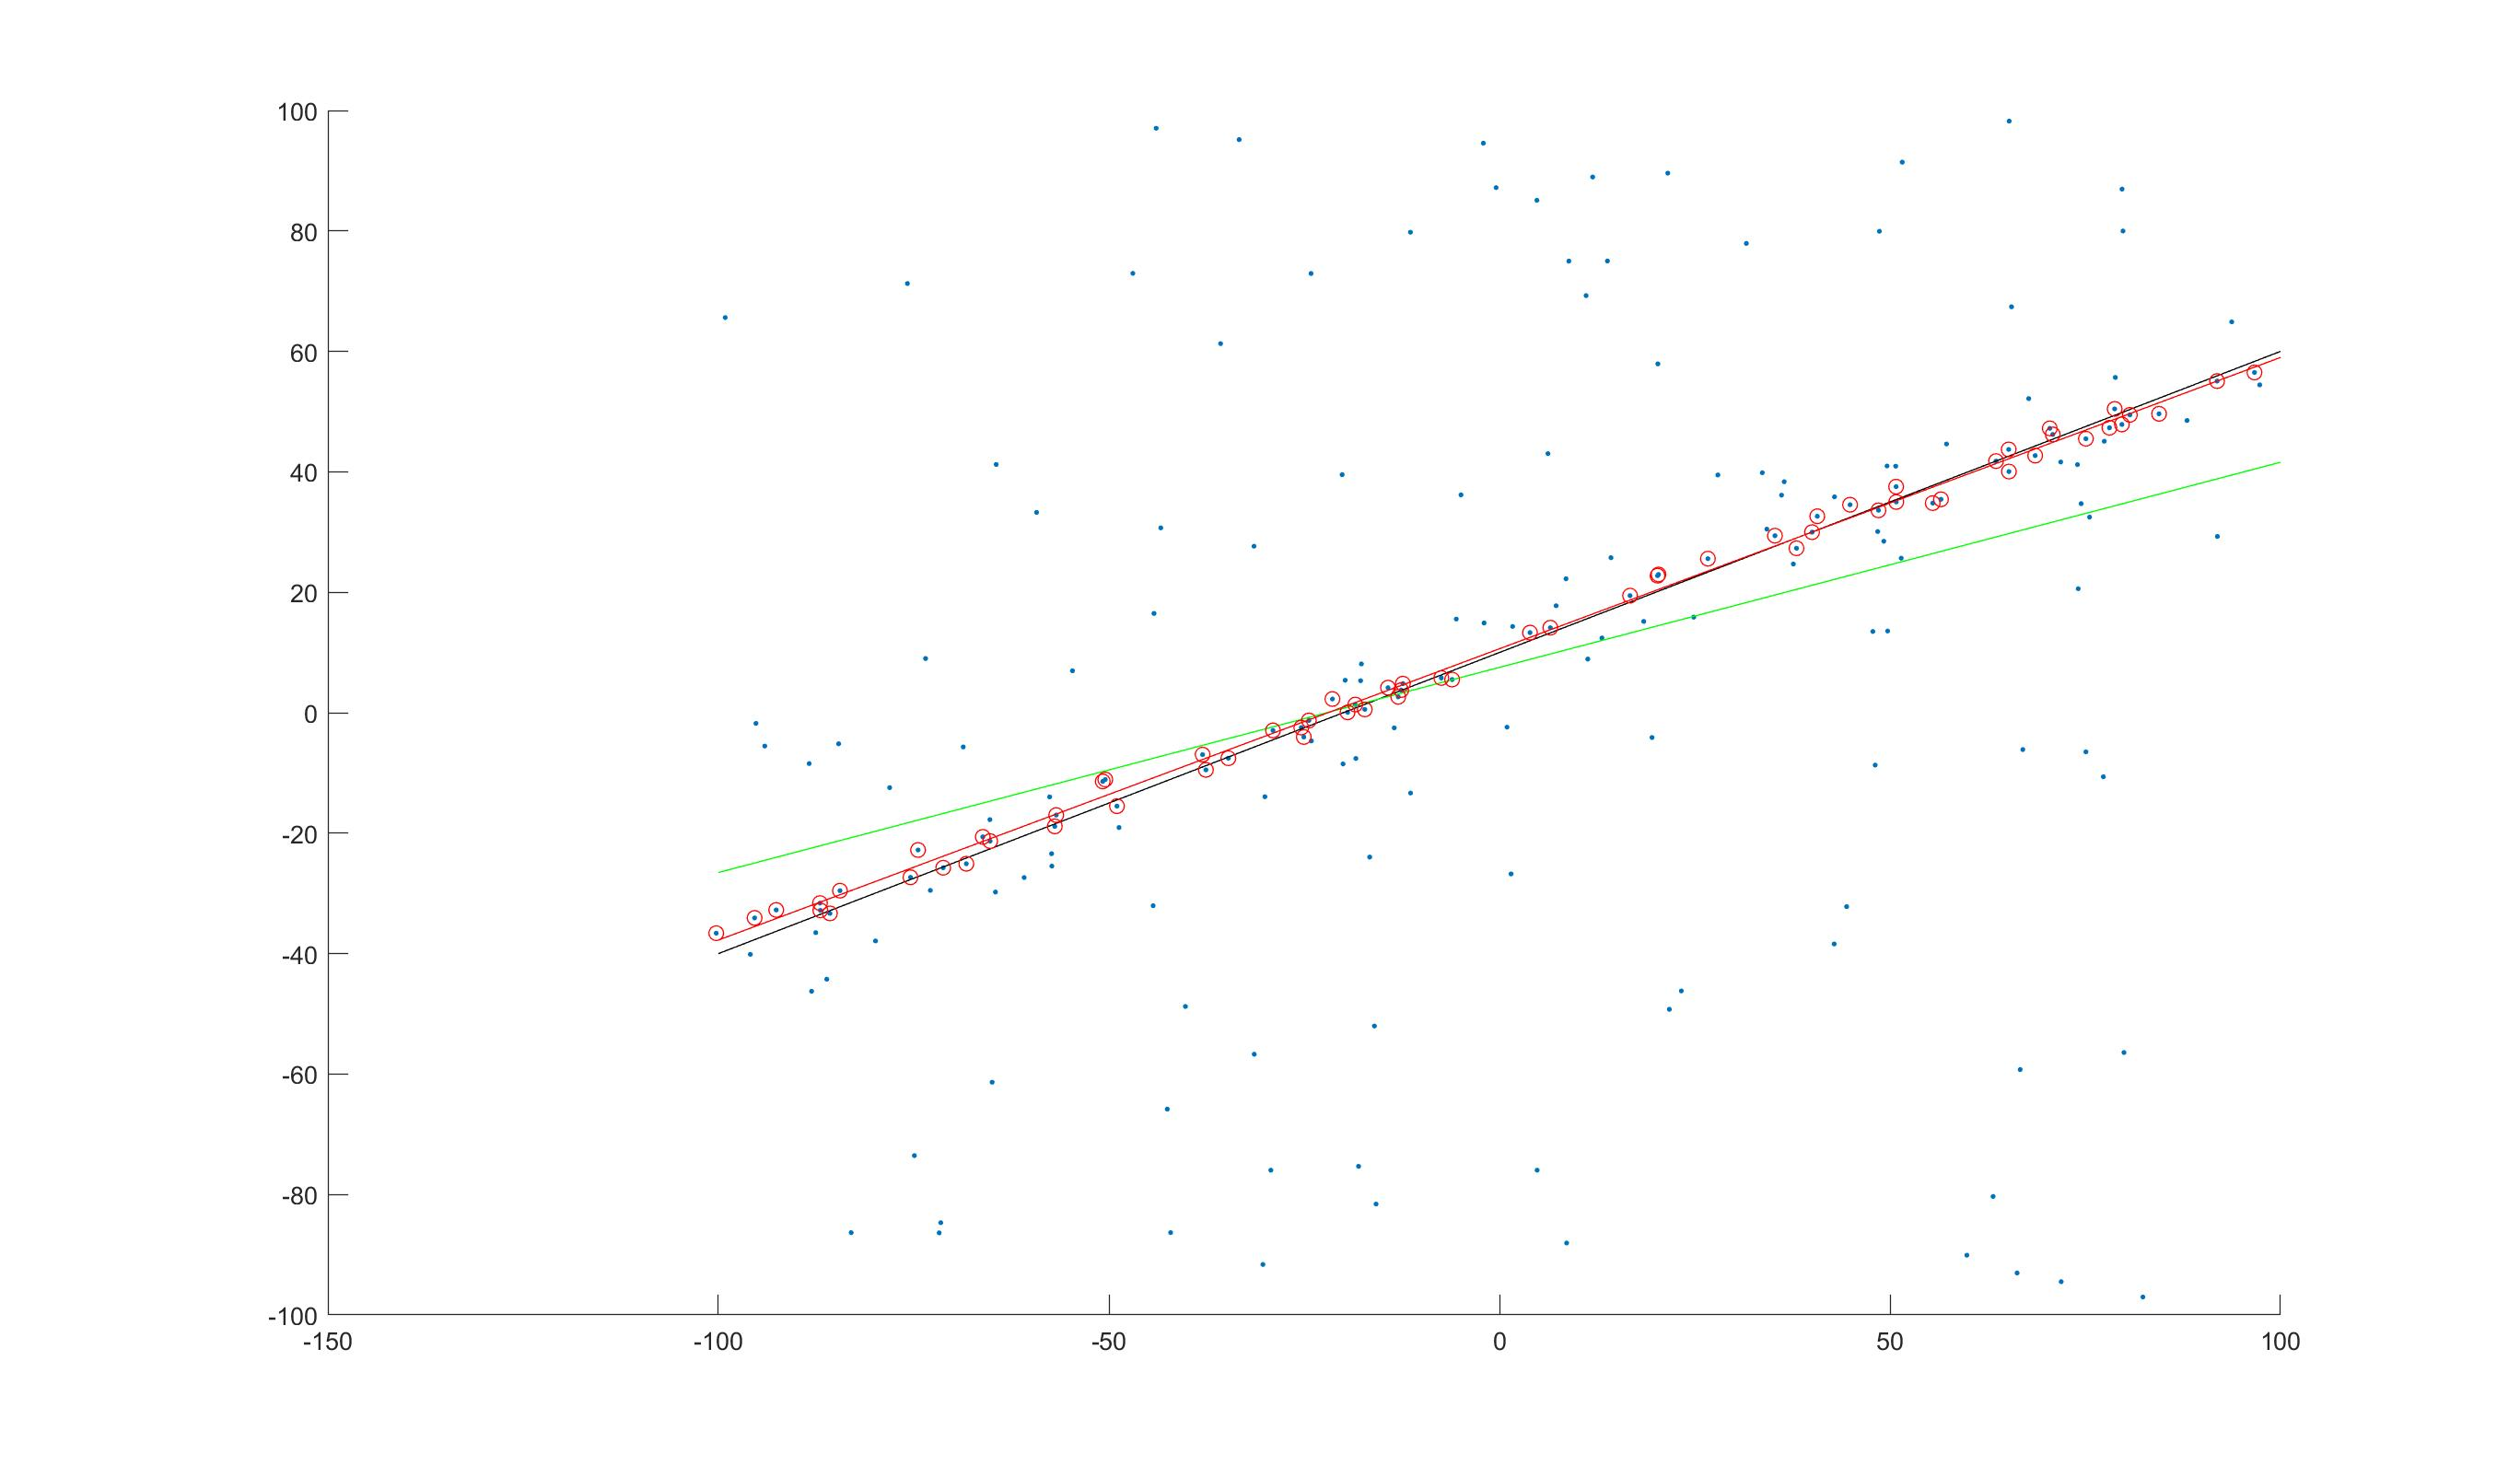
\includegraphics[width=0.9\textwidth]{ransac.jpg}
	\caption{Line Fitting using the RANSAC algorithm}
	\label{fig1}
\end{figure}
\vspace{5mm}
\newline

For the line fitting a random pair of points is choosen from the set of all points with the help of $randperm$. With theese a line going through the two points is calculated. 
\newline
Then the euclidian distance perpendicular to the line is calculated. It was decided to implement this functionality in its own function. 
The inliers are then determined by the set of points, where the distance to the determined line is smaller than the set threshhold. How well the linear line through the two points fits to the given data is simply determined by the amount of inliers. The procedure is then repeated for a set amount of iterations and the model with the largest amount of inliers is choosen as the best representation.  
\newline
The Error values are as follows:
\vspace{5mm}
\newline
$err_{real} = 40.8249$
\vspace{5mm}
\newline
$err_{ls} = 92.7829$
\vspace{5mm}
\newline
$err_{ransac} =41.5313$
\vspace{5mm}
\newline

As can be seen the RANSAC algorithm performs very well even in case of a lot of noise and outlier points in the dataset. 

\section{Fundamental Matrix Estimation}

\vspace{5mm}
\newline
\begin{figure}[ht]
	\centering
	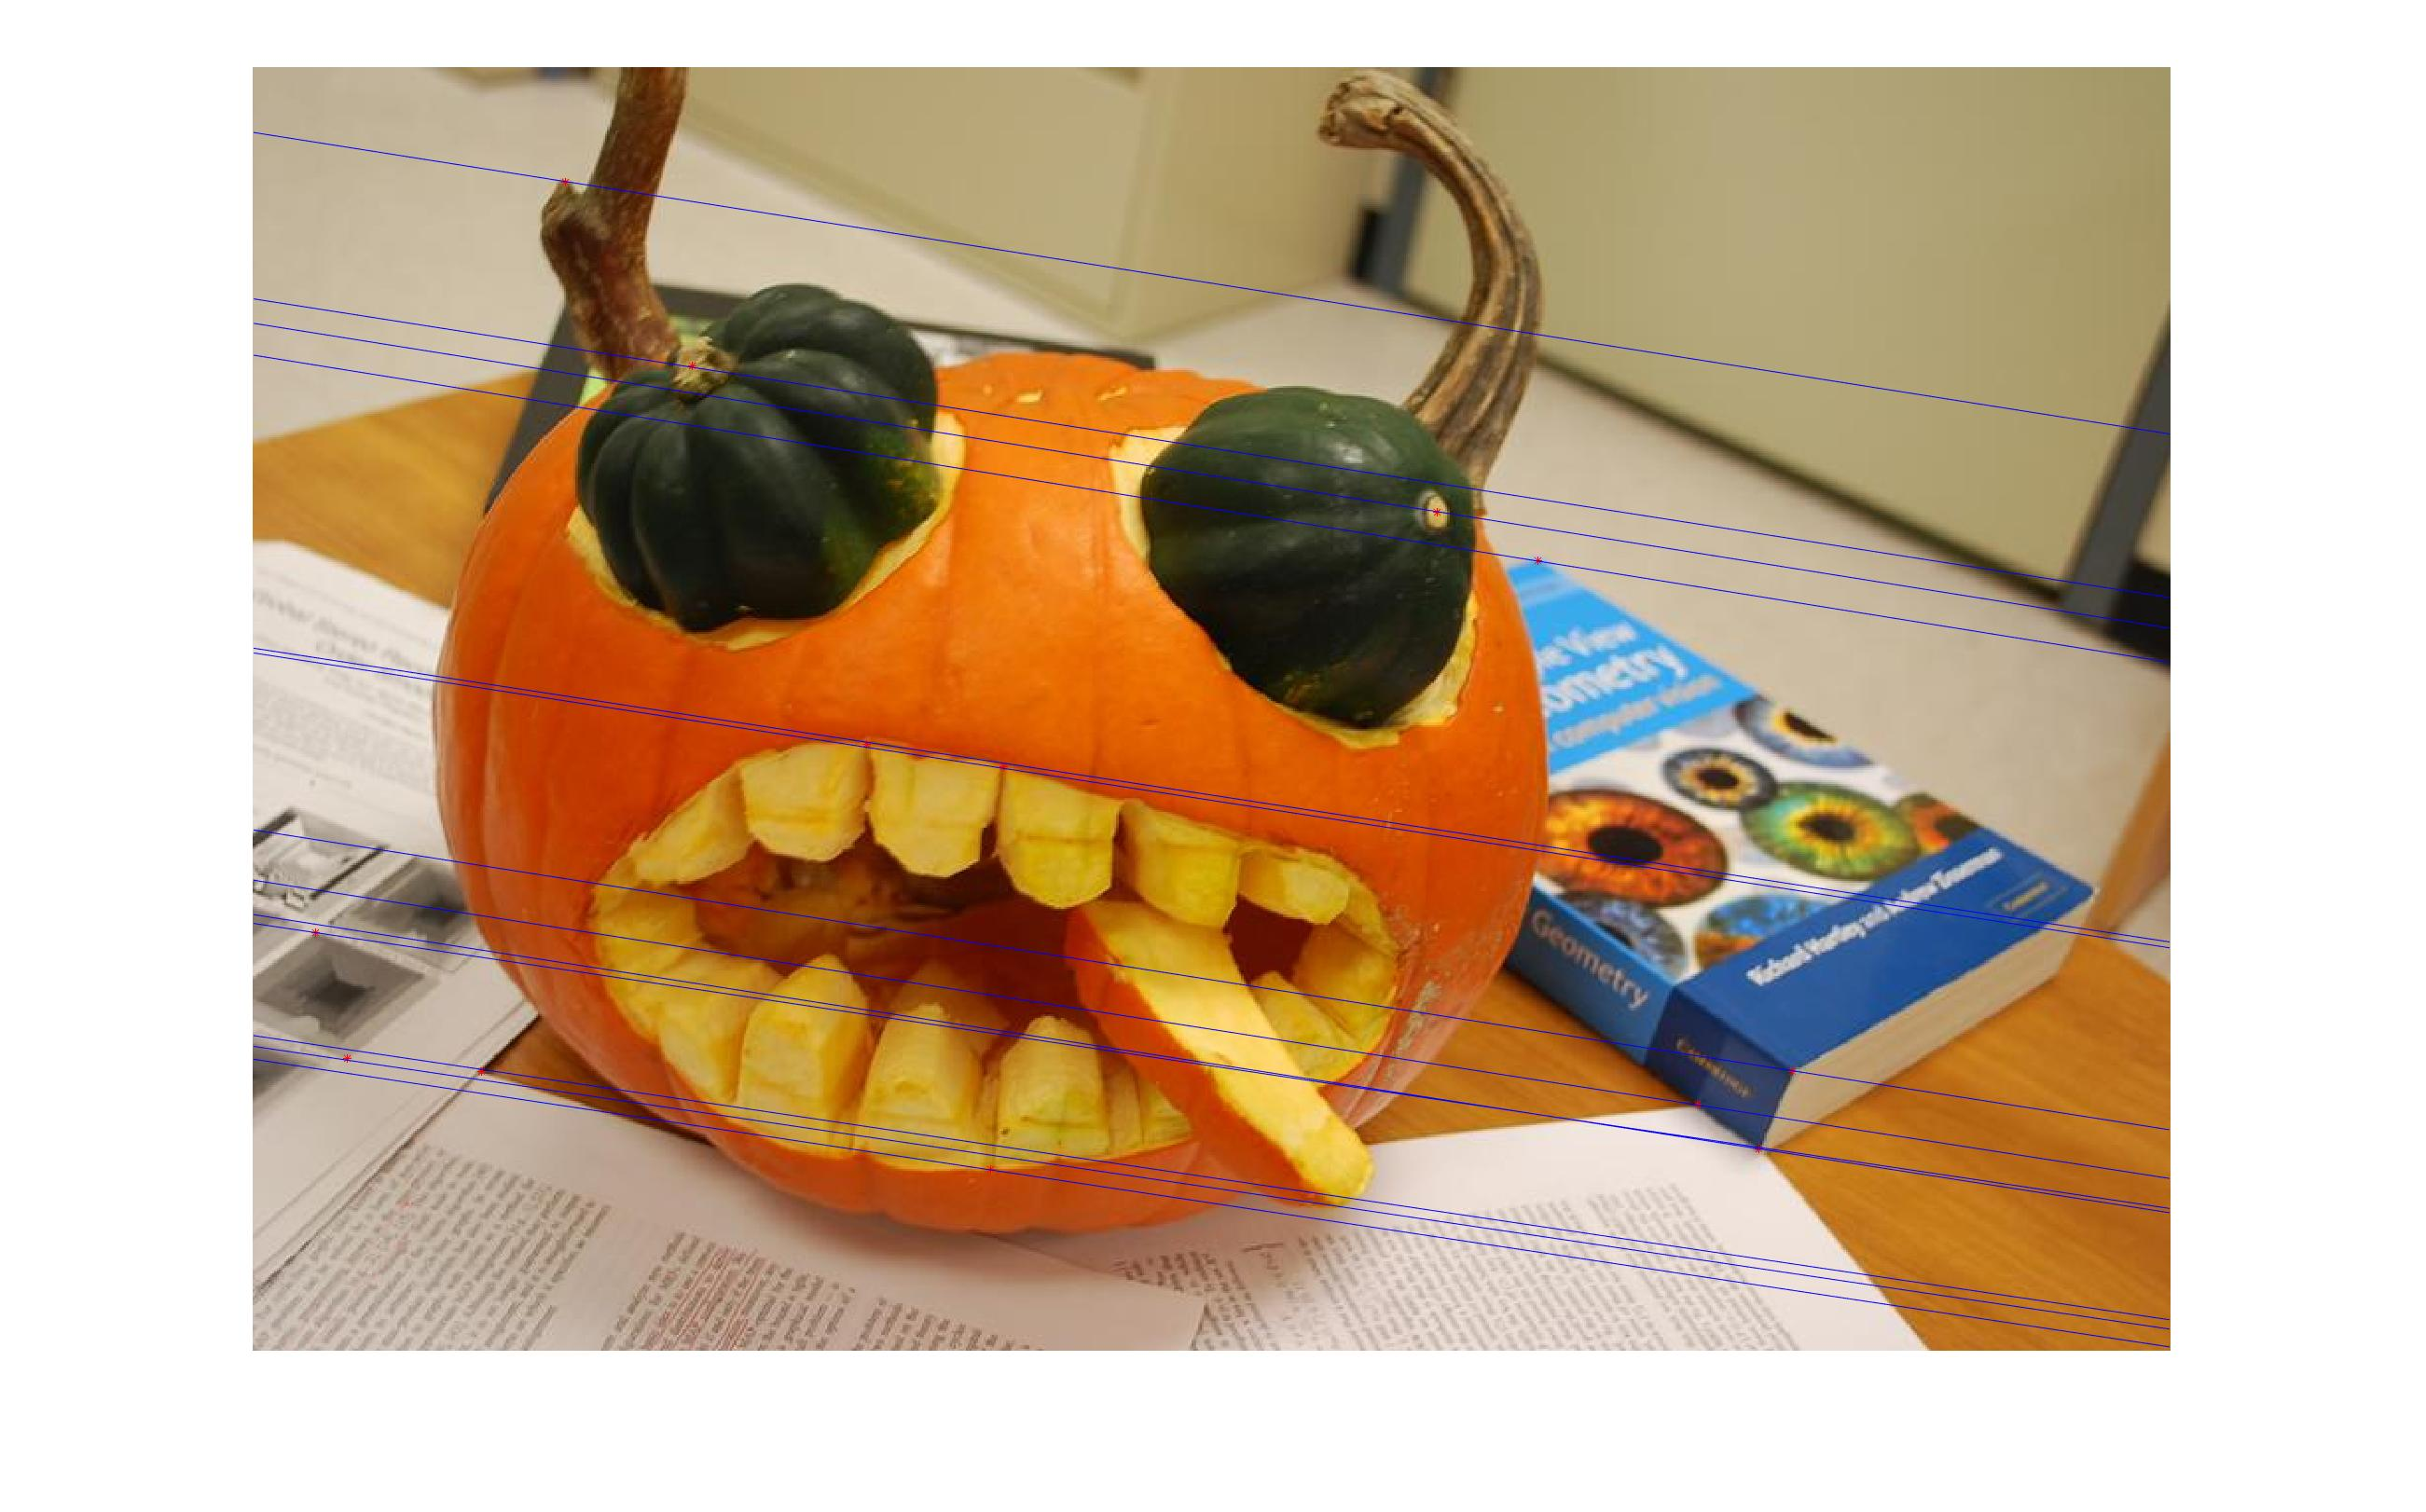
\includegraphics[width=0.8\textwidth]{F1Pumkin.jpg}
	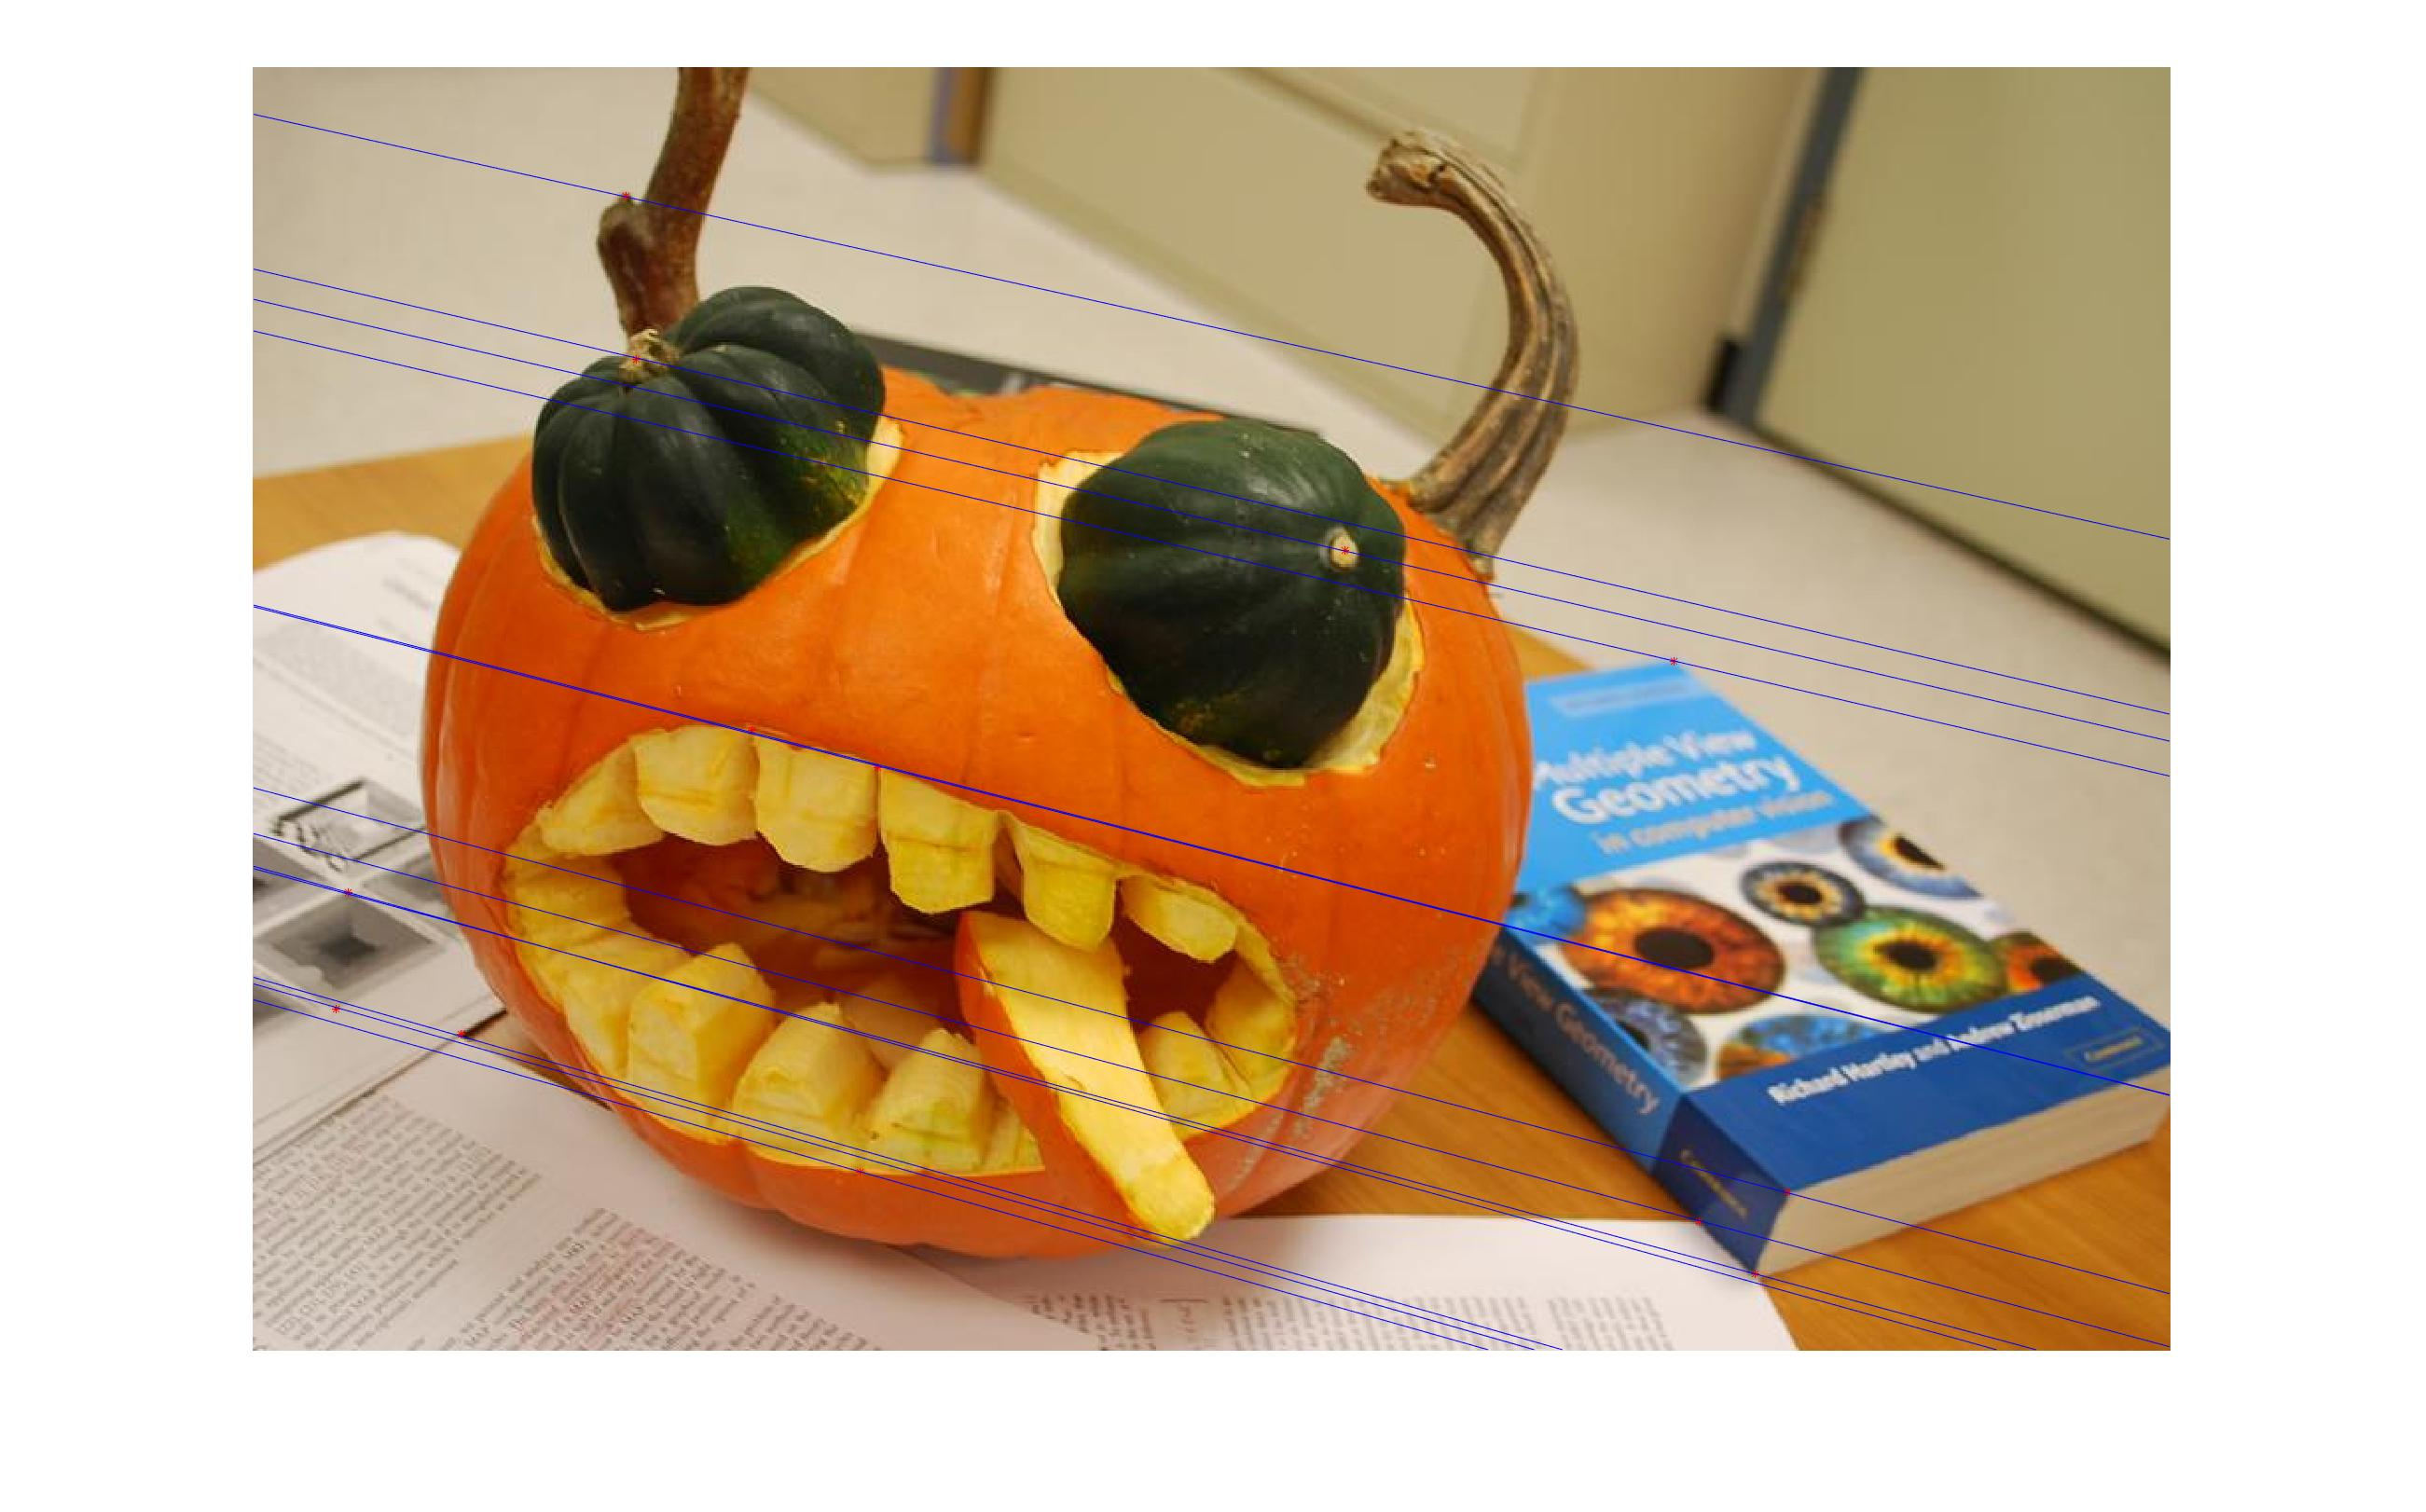
\includegraphics[width=0.8\textwidth]{F2Pumkin.jpg}
	\caption{Fundamental matrix estimation without enforced zero determinante}
	\label{fig1}
\end{figure}
\vspace{5mm}
\newline

\begin{figure}[ht]
	\centering
	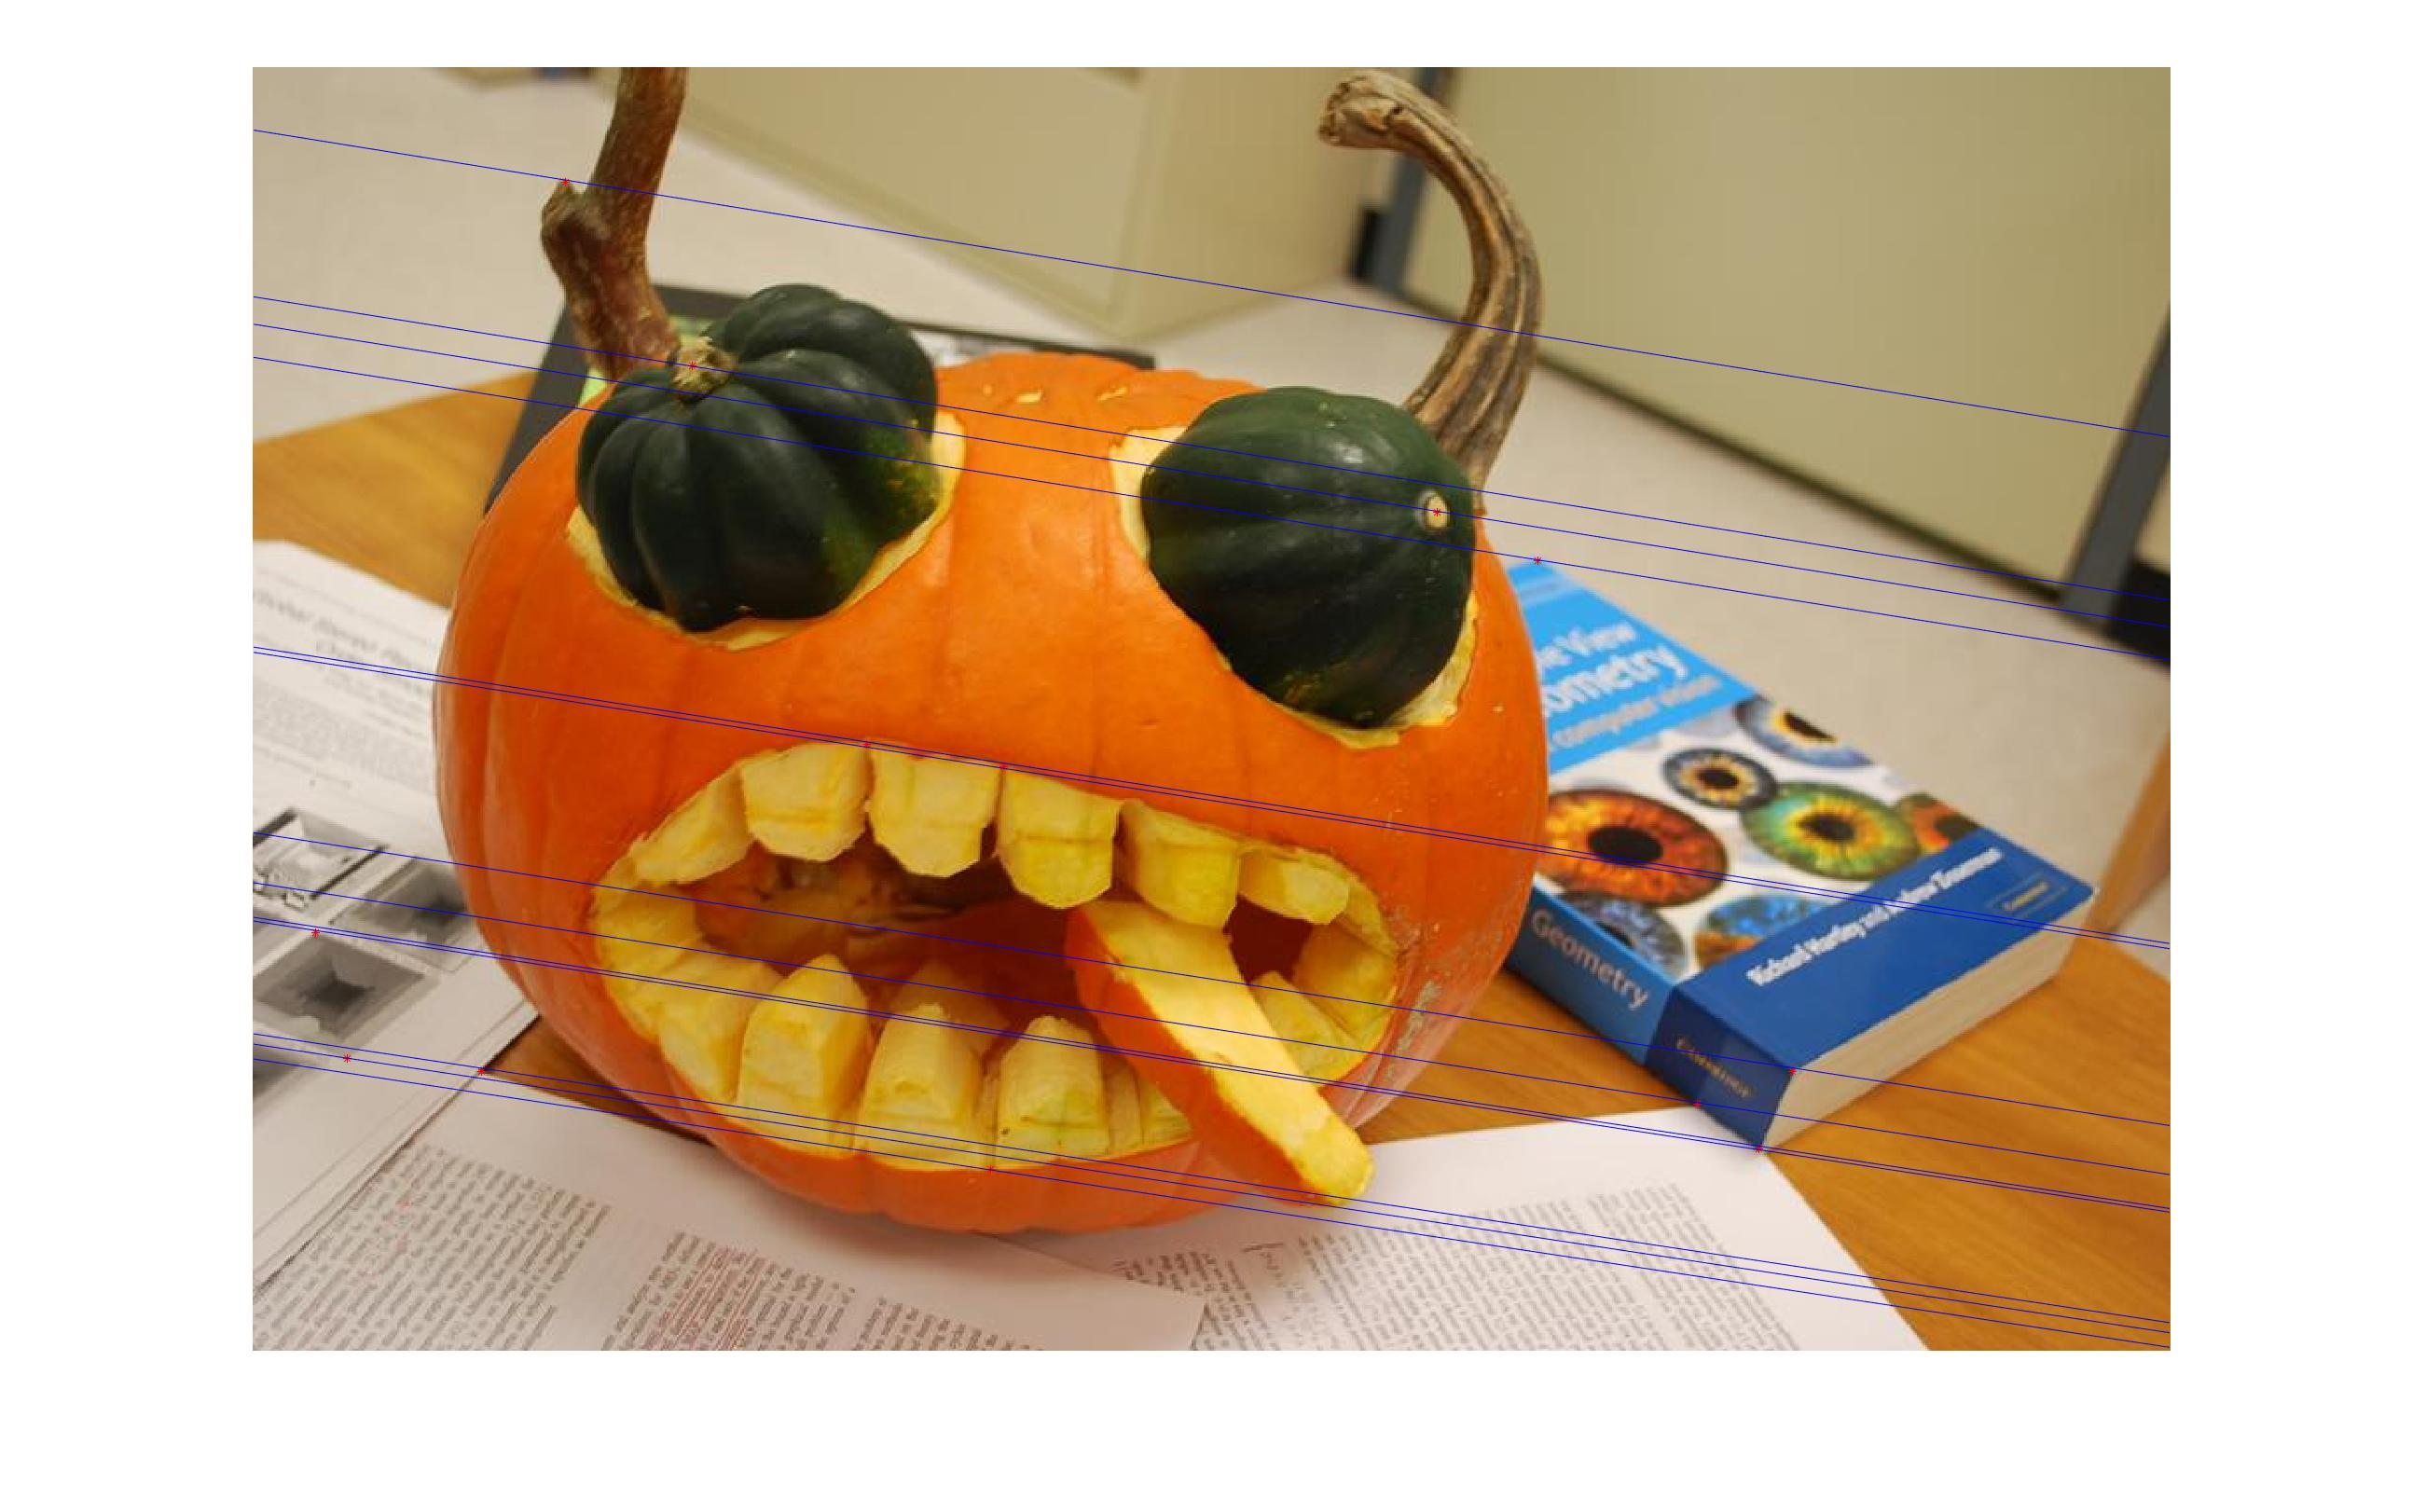
\includegraphics[width=0.8\textwidth]{Fh1Pumkin.jpg}
	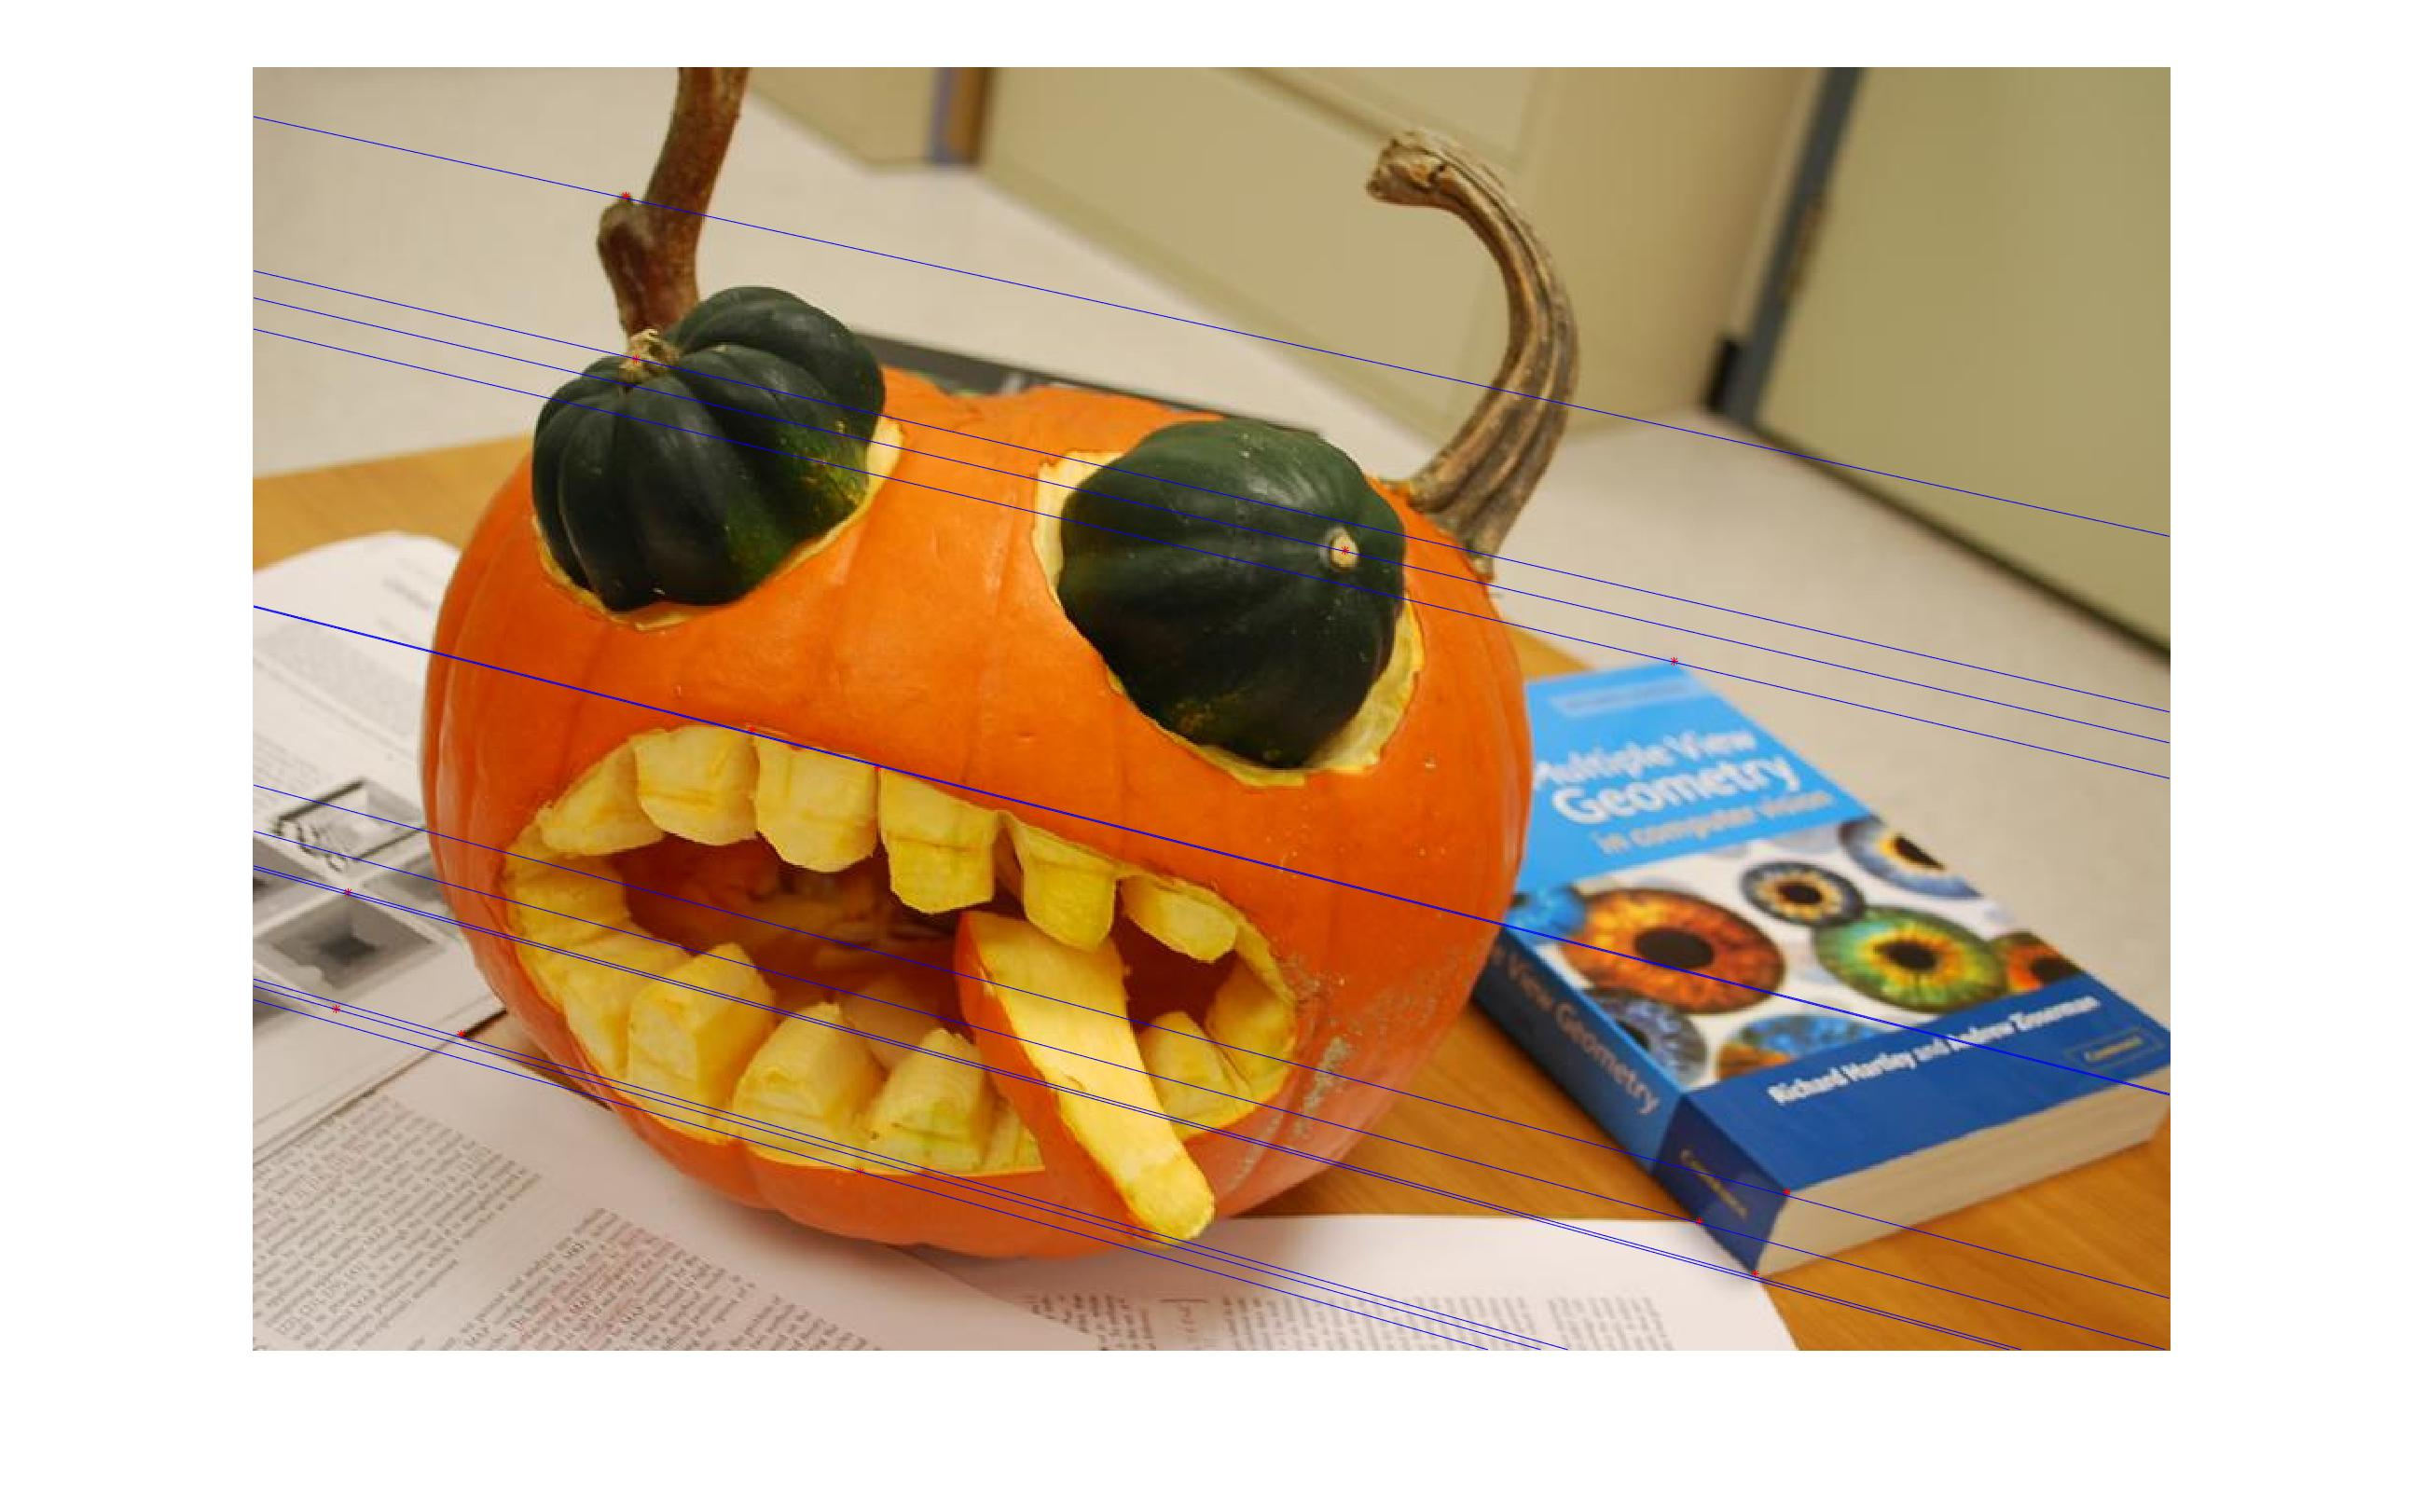
\includegraphics[width=0.8\textwidth]{Fh2Pumkin.jpg}
	\caption{Fundamental matrix estimation with enforced zero determinante}
	\label{fig1}
\end{figure}
\vspace{5mm}
\newline

\begin{figure}[ht]
	\centering
	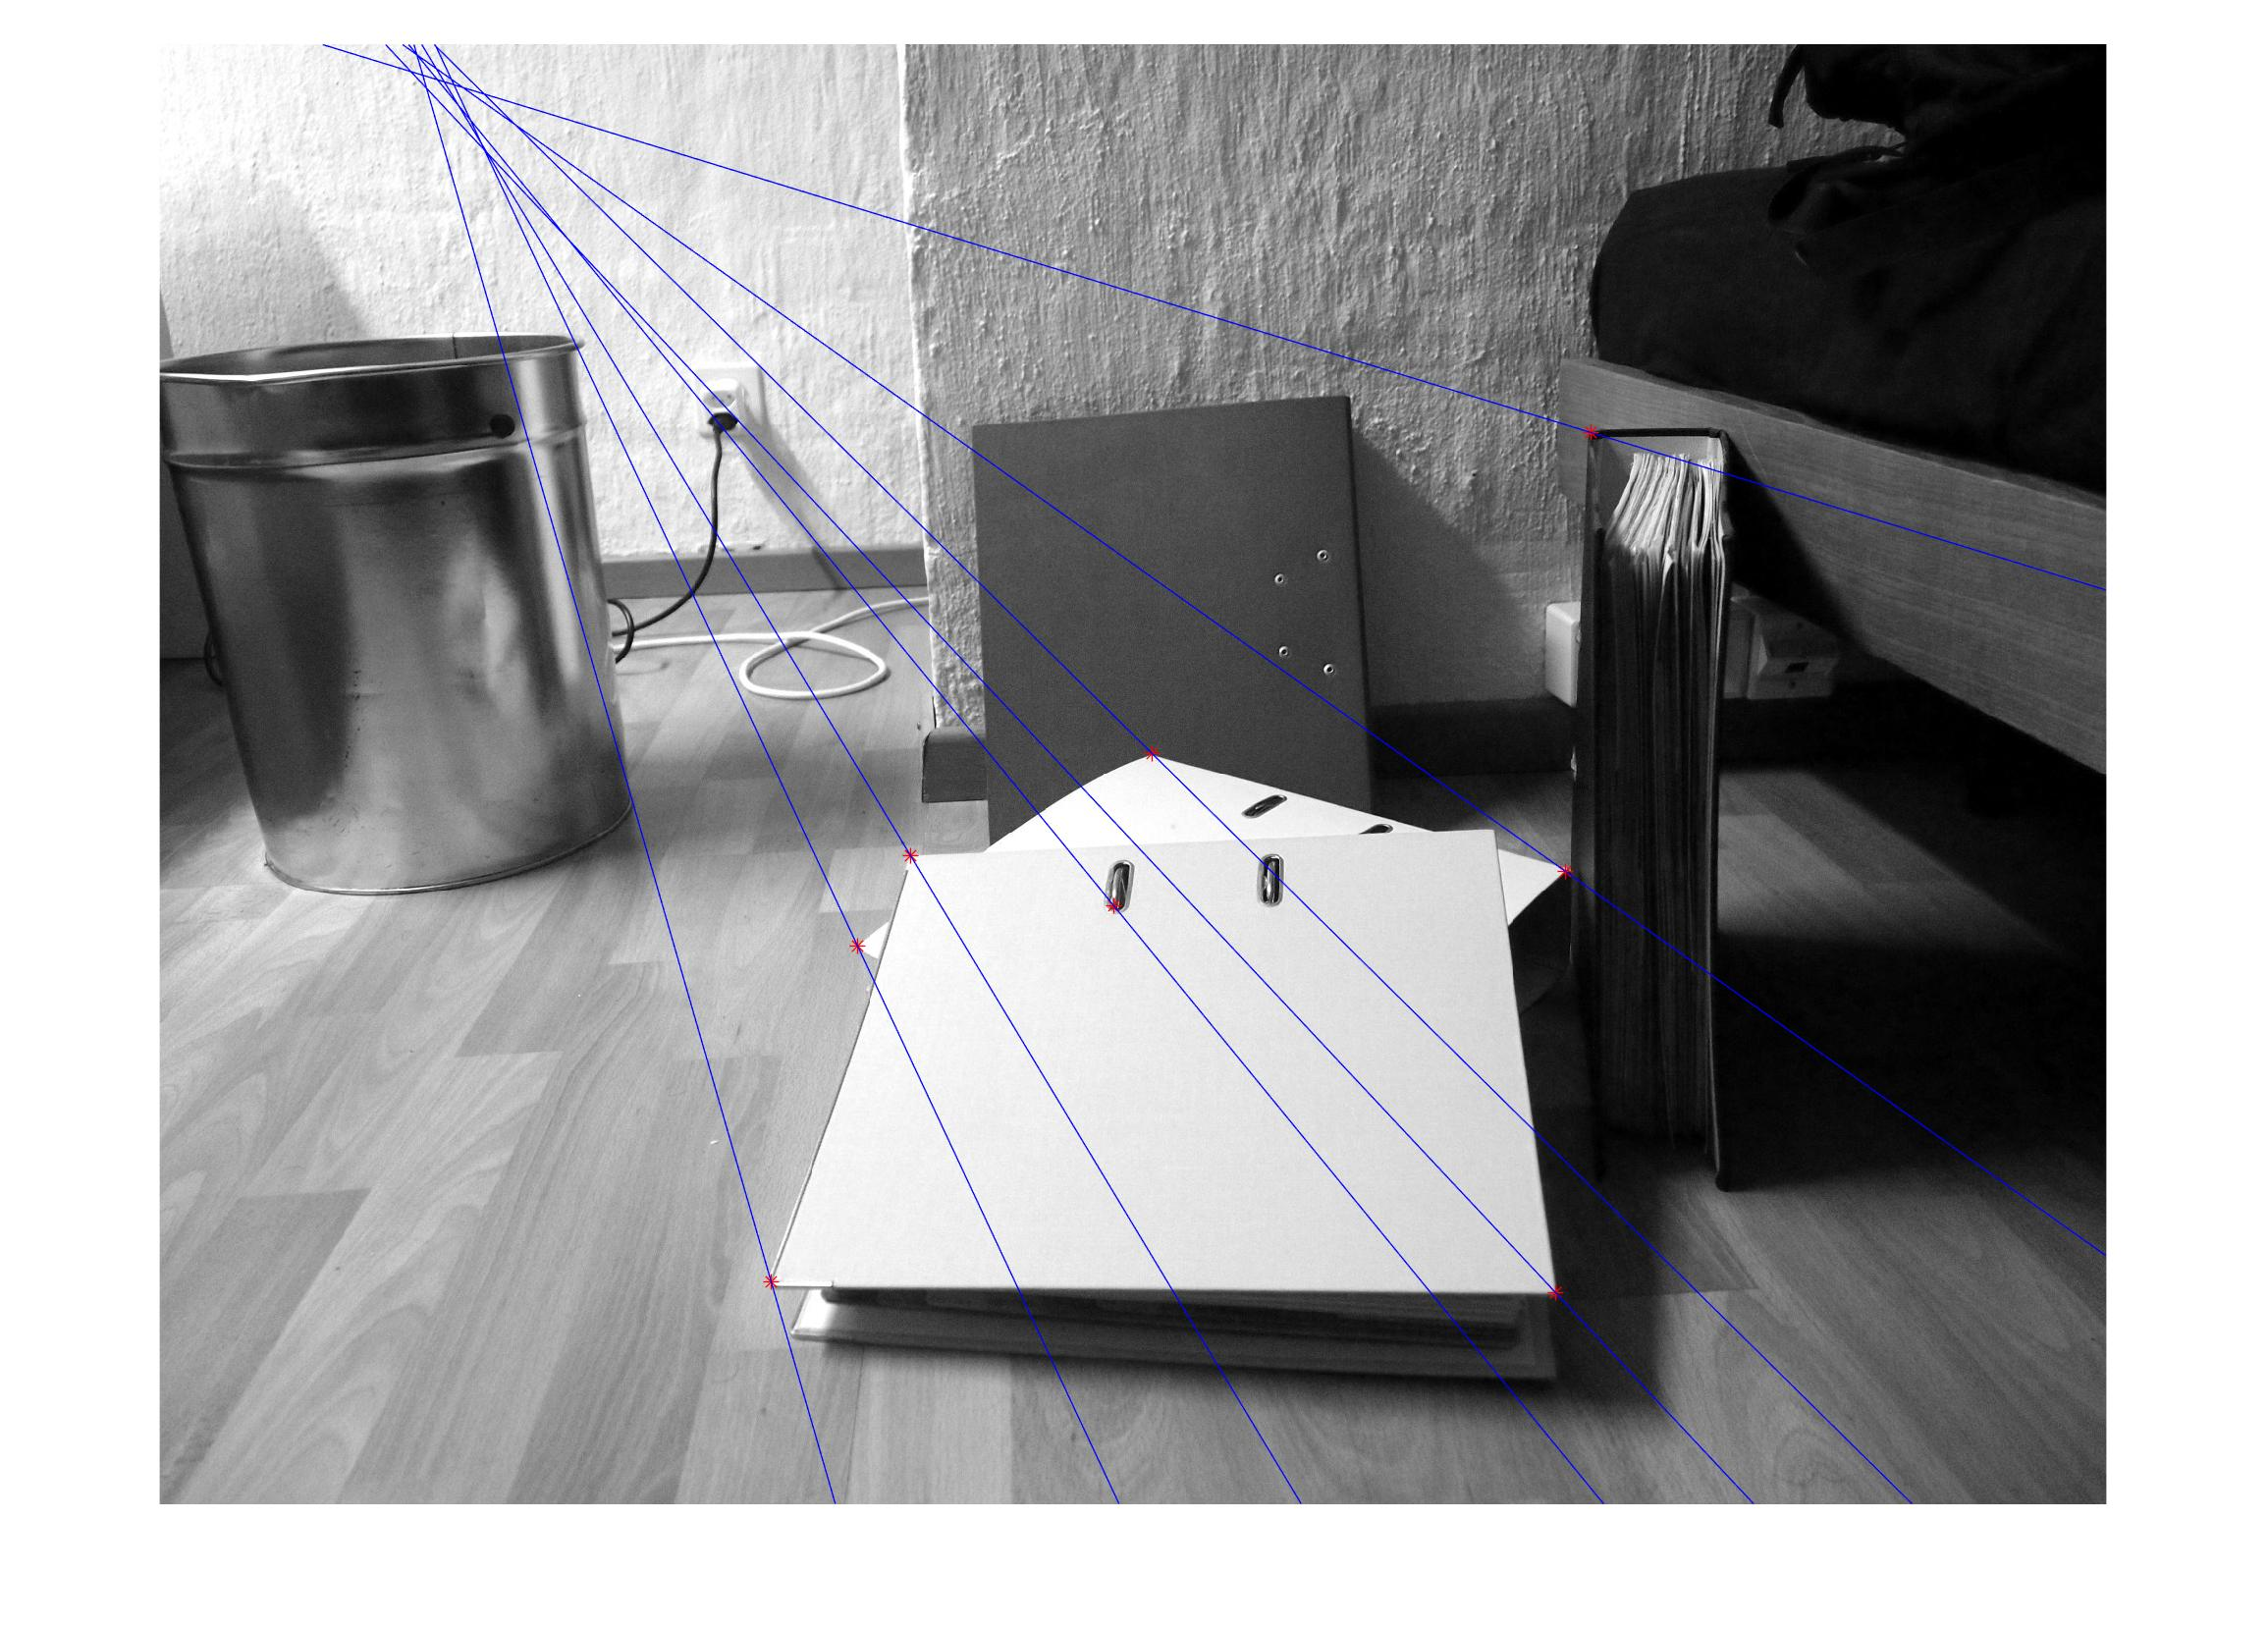
\includegraphics[width=0.8\textwidth]{F1Book.jpg}
	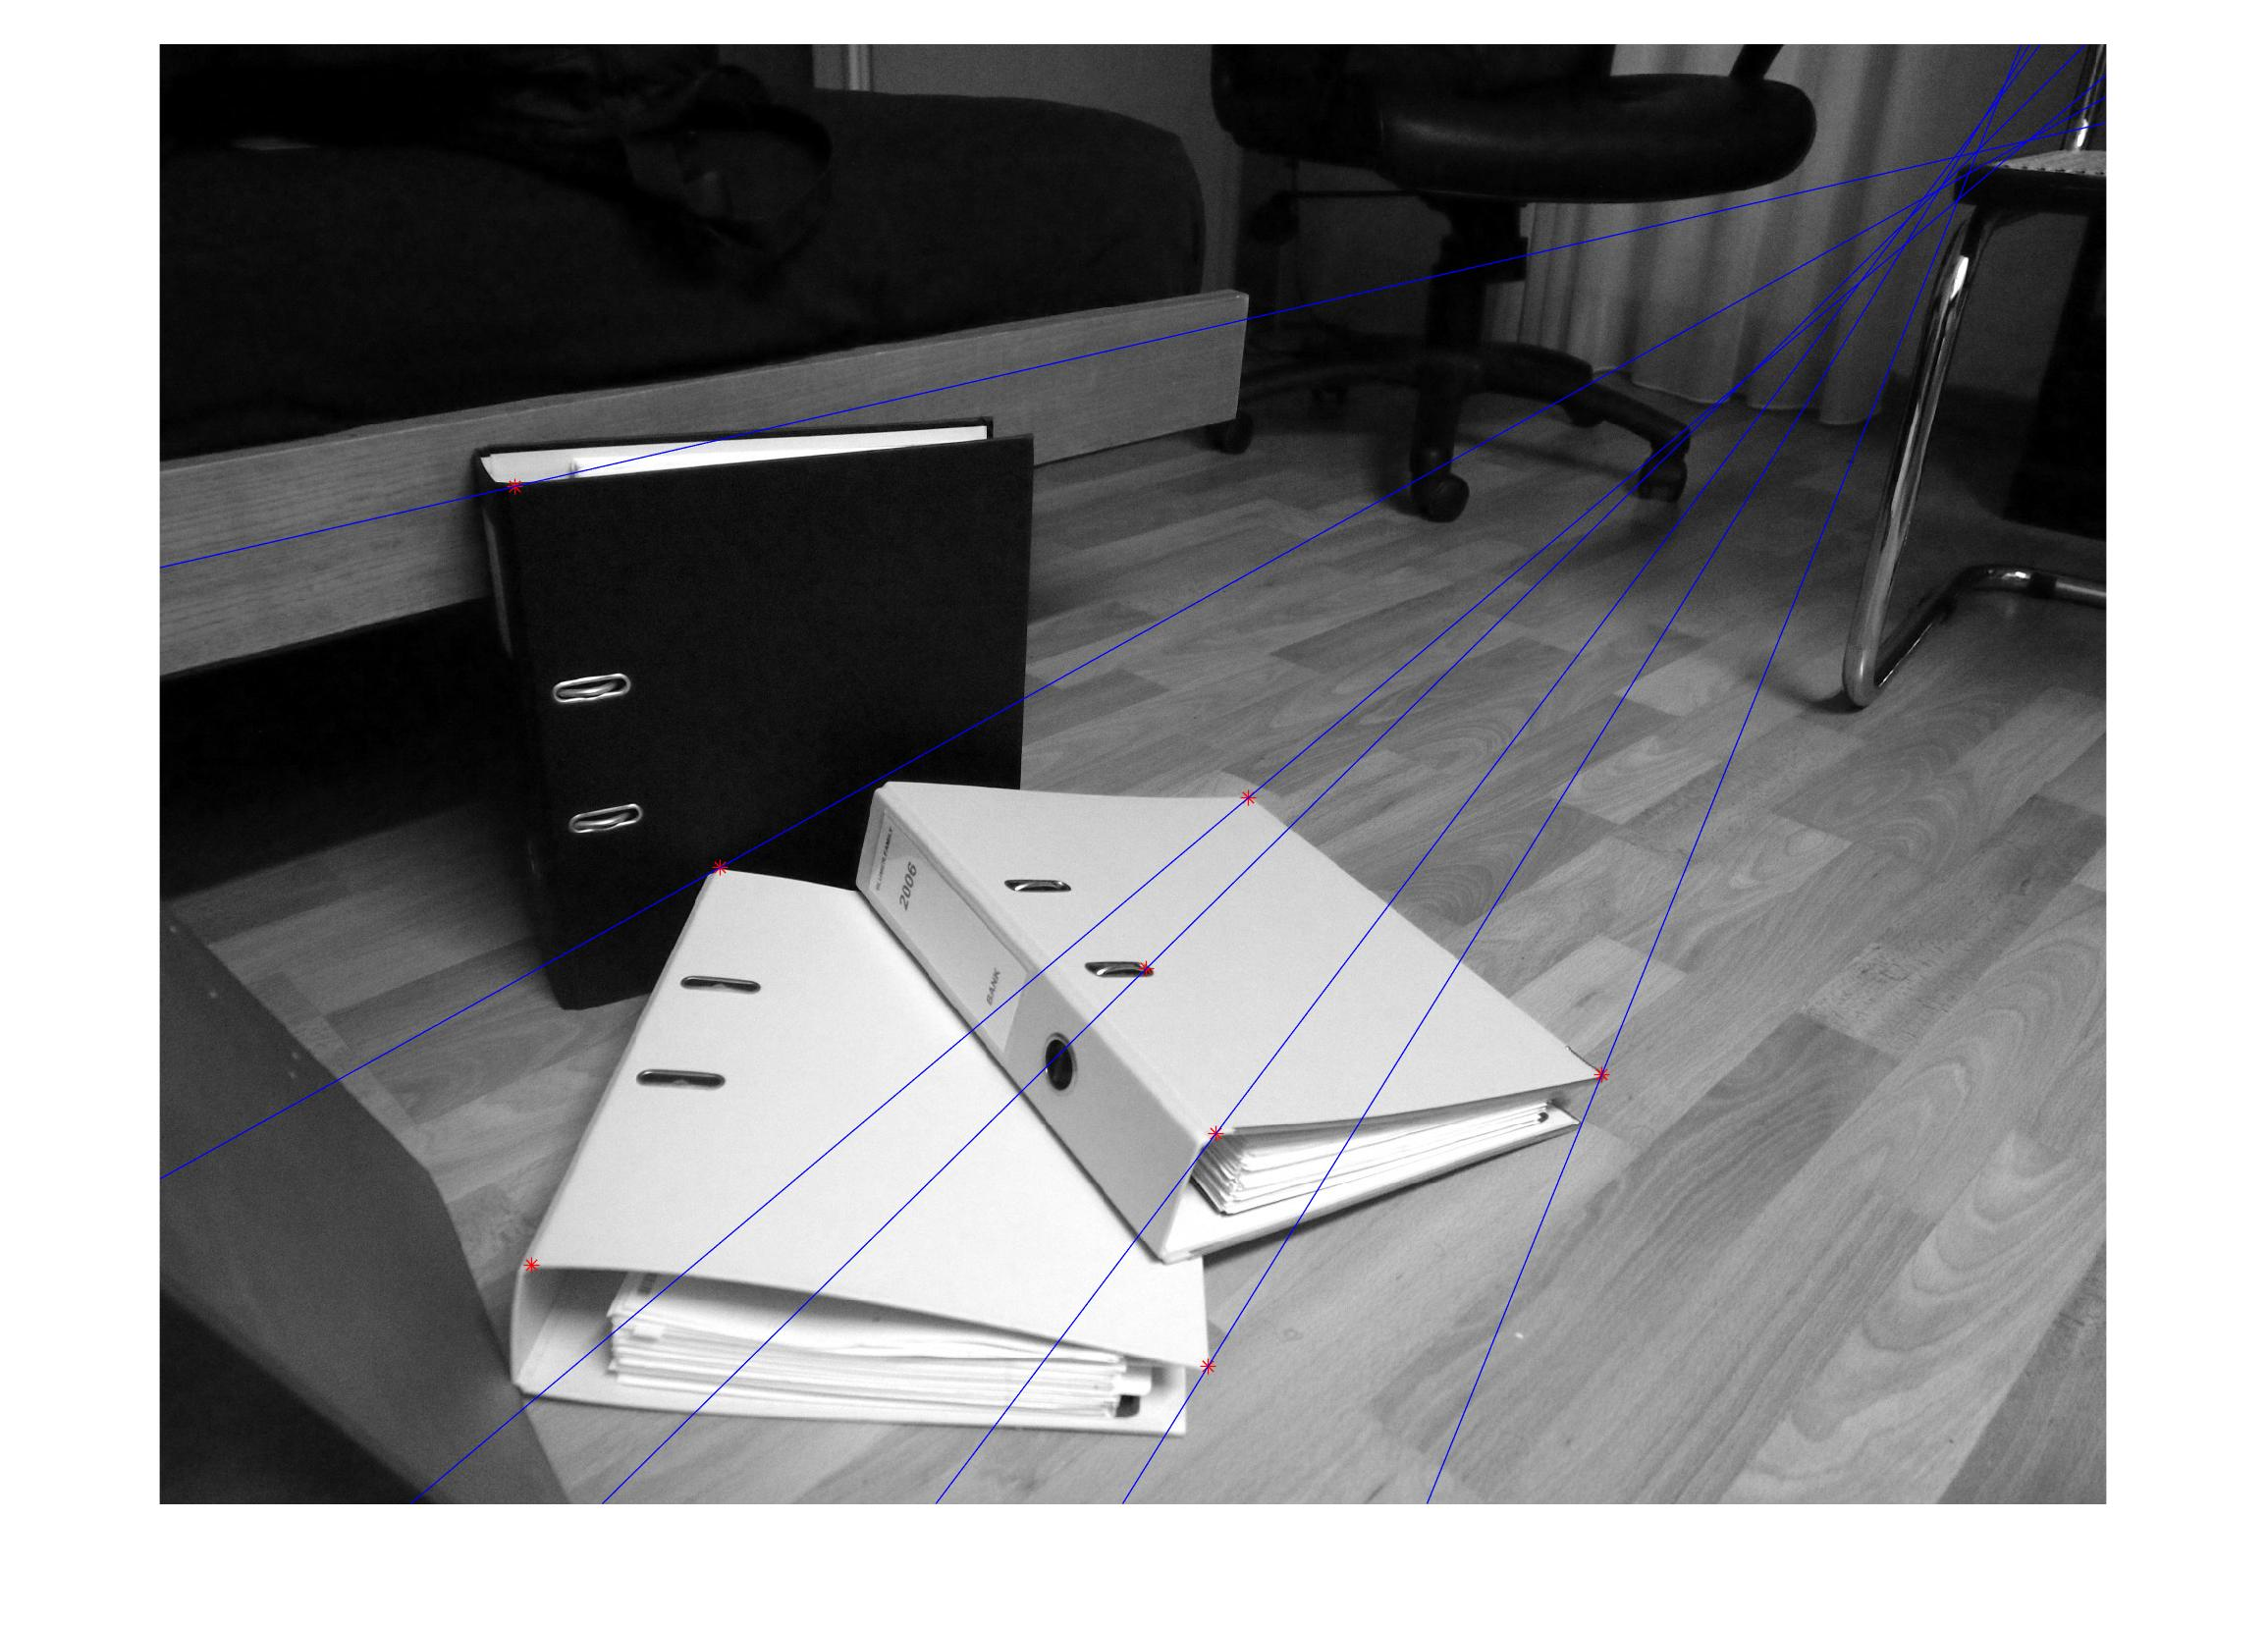
\includegraphics[width=0.8\textwidth]{F2Book.jpg}
	\caption{Fundamental matrix estimation without enforced zero determinante}
	\label{fig1}
\end{figure}
\vspace{5mm}

\newline
\begin{figure}[ht]
	\centering
	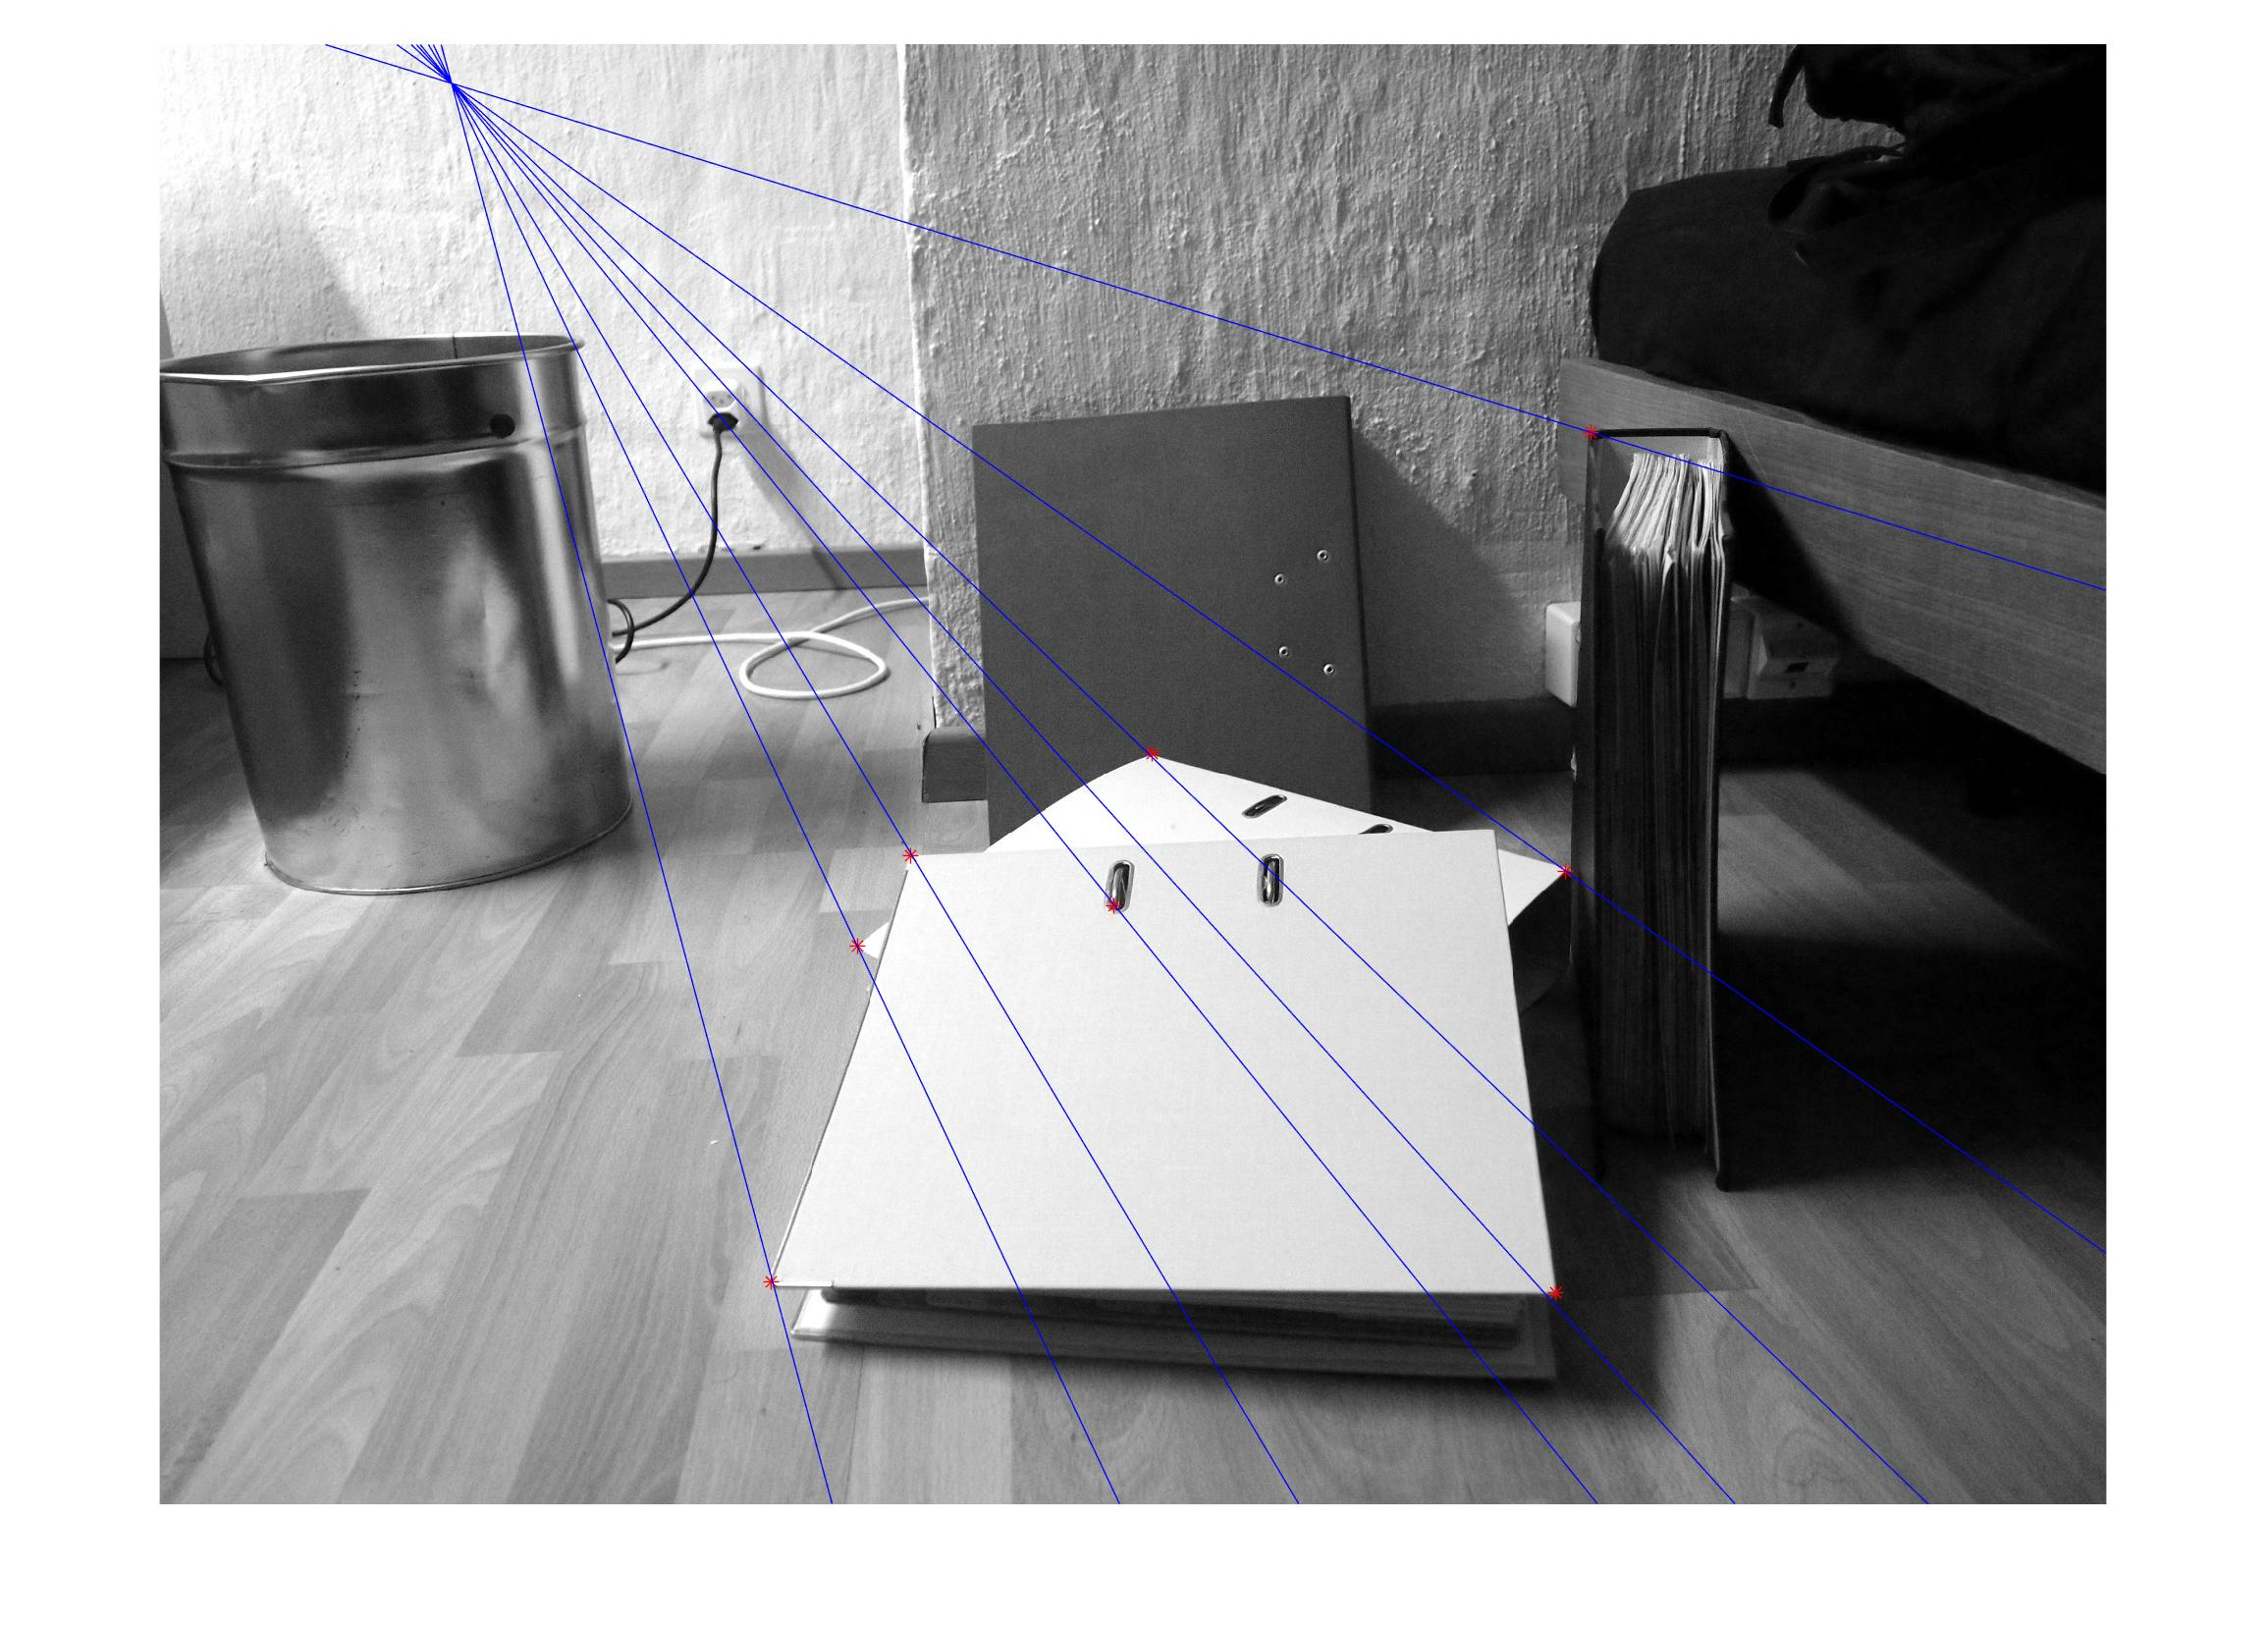
\includegraphics[width=0.8\textwidth]{Fh1Book.jpg}
	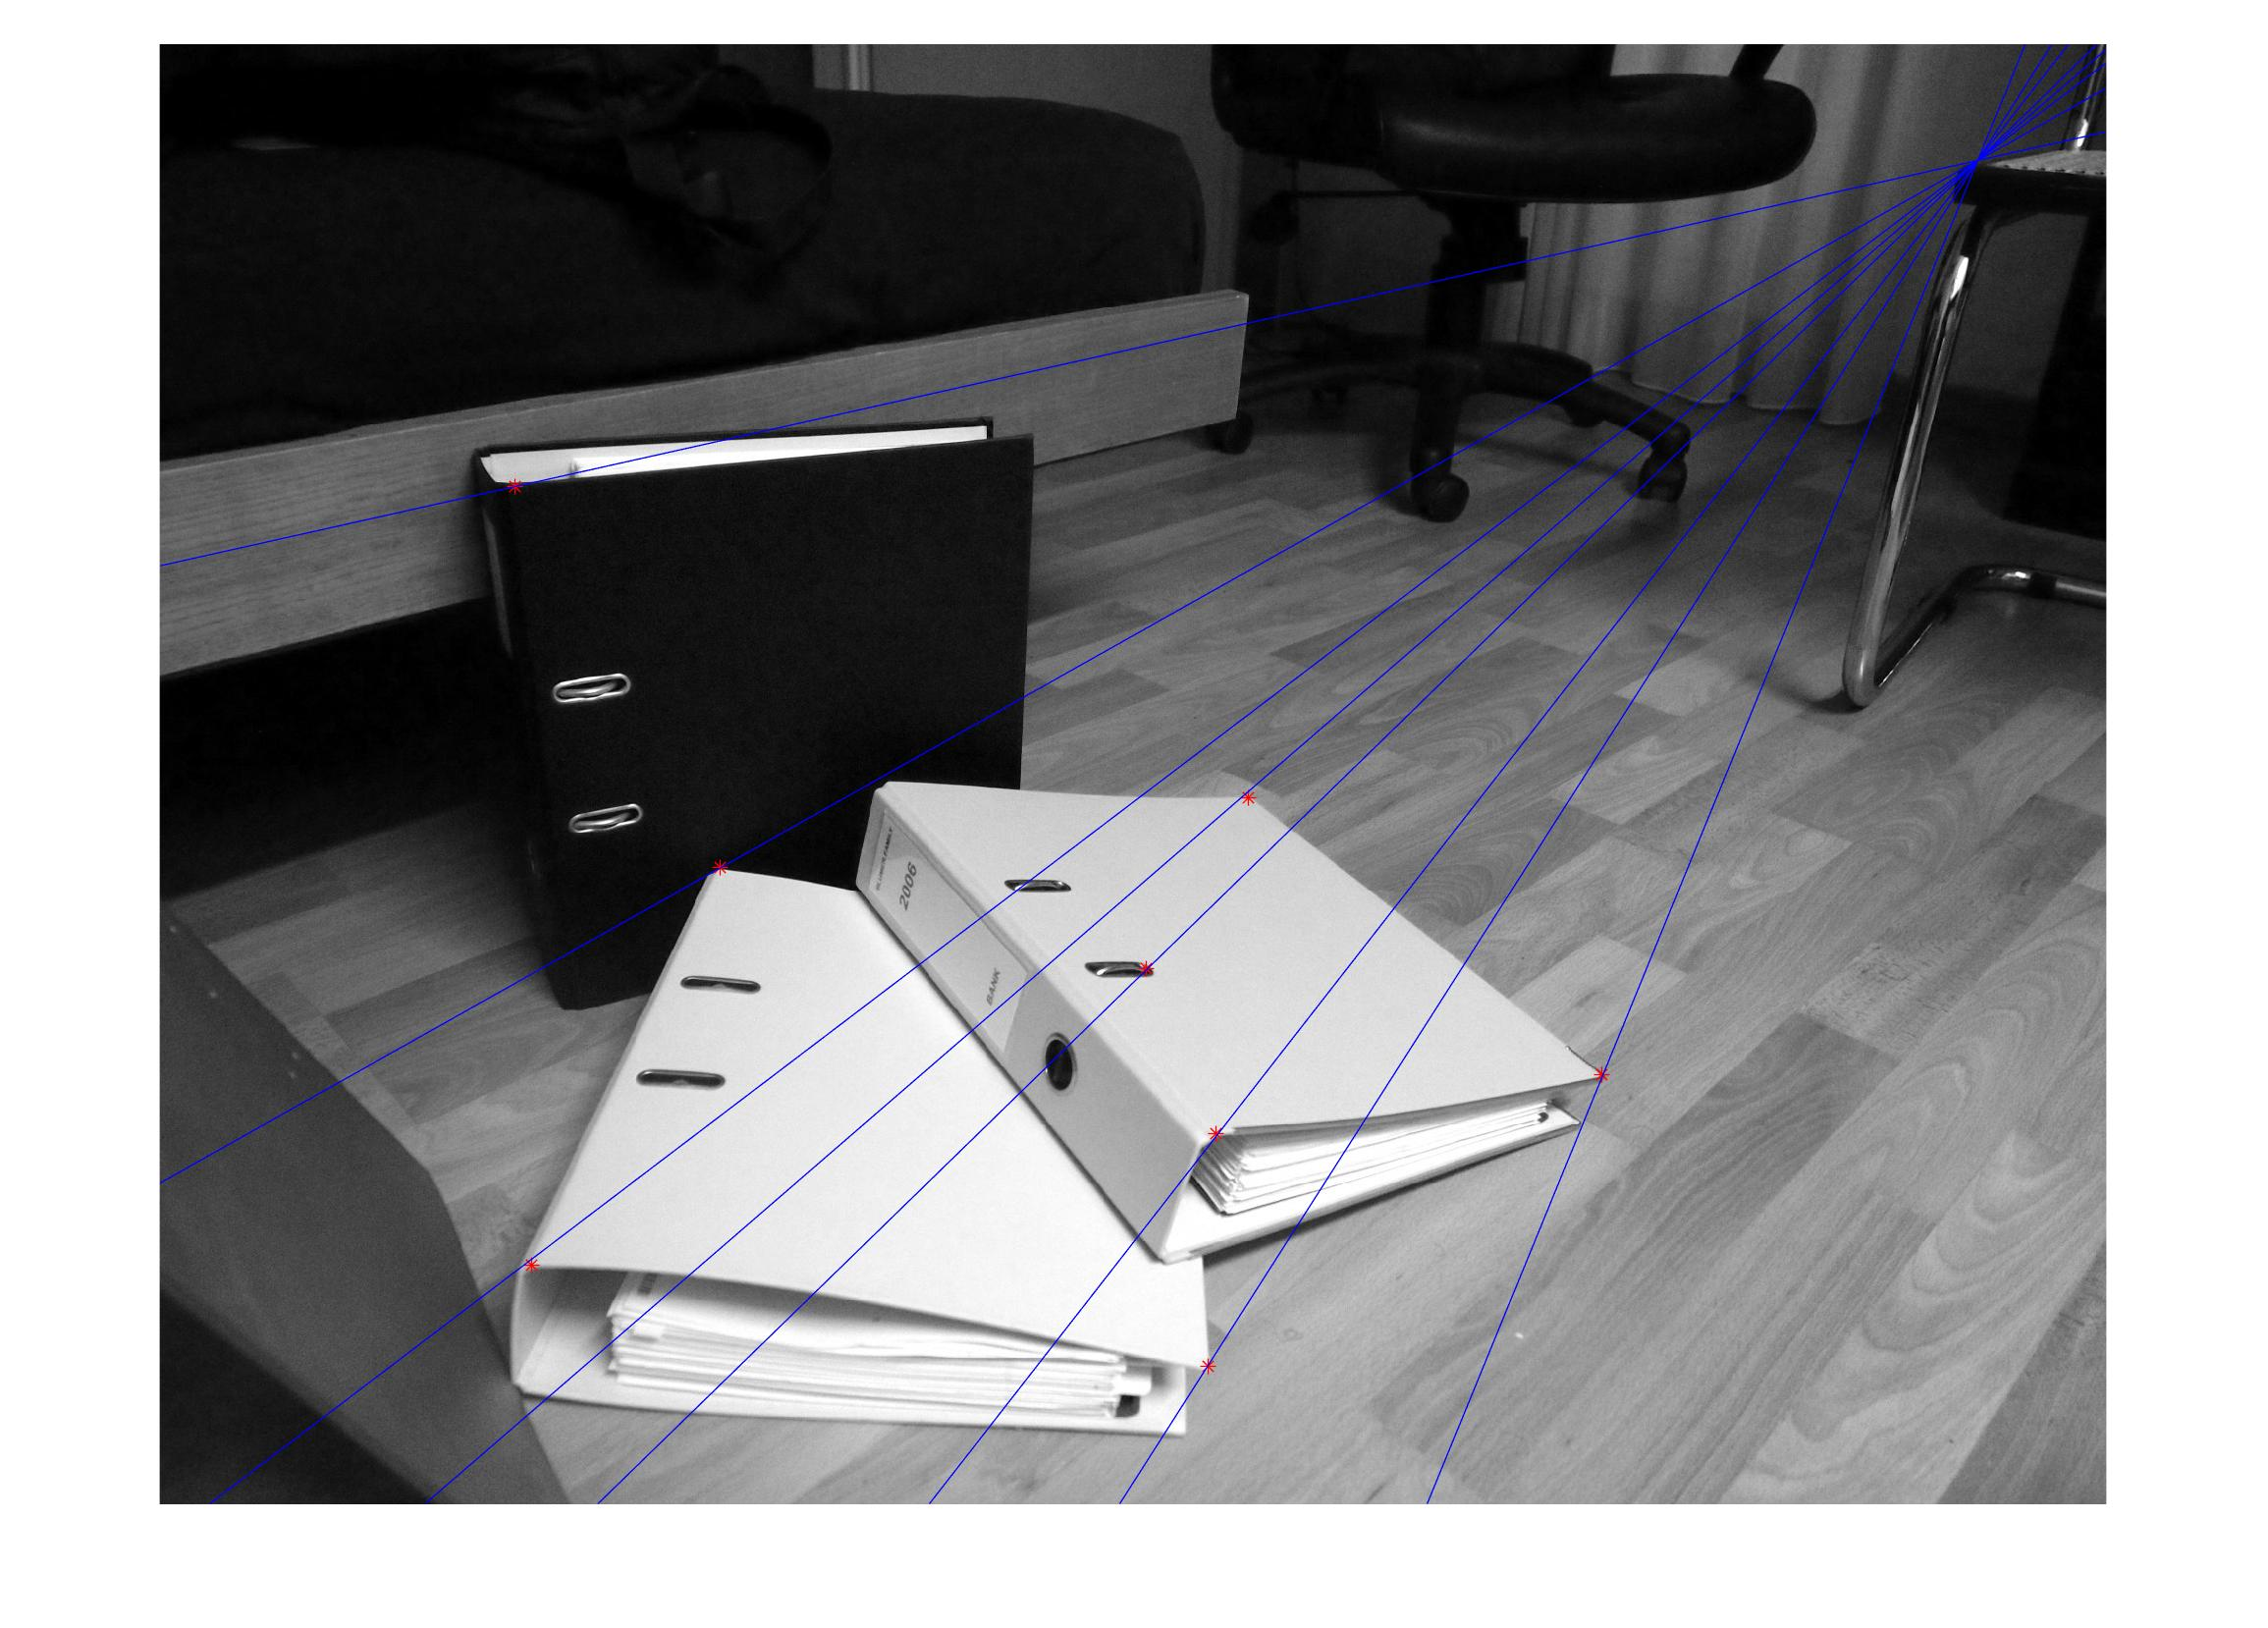
\includegraphics[width=0.8\textwidth]{Fh2Book.jpg}
	\caption{Fundamental matrix estimation with enforced zero determinante}
	\label{fig1}
\end{figure}
\vspace{5mm}
\newline

To estimate the fundamental matrix a set of min. eight point pairs from two images was chossen. First the points are normalized as described in the delivered paper. 
From the normalized pairs of points a matrix of equations can be contructed where each row is comprised of: 
\vspace{5mm}
\newline
$(x'*x, y'*x, x, x'*y, y'*y, y,x',y',1)$
\vspace{5mm}
\newline

This matrix A is then used to solve the equation:
\vspace{5mm}
\newline
$A*vec(F)=0$
\vspace{5mm}
\newline

Since this system of equation is not invertible we use the trick of single value decomposition. The smallest eigenvalue of A fullfills this set of equations with the smallest possible error since the scaling of the vector will be almoust zero. The corresponding eigenvector is the fundamental matrix in vectorized form. Note that the $svd$ function of matlab already results in a normalized eigenvector. 
\newline
To additionally enforce the contraint of a determinante equal to zero the fundamental matrix F is decomposed again and its third eigenvalue is set to zero. As a last step the denormalization is applied. 
\vspace{5mm}
\newline
As can be seen especially in the images $rect1$ and $rect2$ the epipoles are in the point where all the epipolar lines intersect. As can be seen the enforcing of the zero determinante results in the eplipolar lines tracking the corresponding points slightly worse. On the other hand this results in the epipolar lines exactly intersecting in the epipoint. 



\section{Feature Extraction and Matching}
VLFEAT was installed as described on the website.
\vspace{5mm}

\section{Eight-point RANSAC}

The eight point RANSAC algorithm is a combination between the normal ransac algorithm and the fundamental matrix estimation. Here the fundamental matrix is estimated by eight randomly selected points. The performance of the randomly choosen points is the determined by the number of inliers. for these inliers the sampson error (which is not the real sampson error but the equation given in the exercise) is smaller than a given threshhold. Again by performing many iterations a good solution can be found. 
\vspace{5mm}
\newline
For additional efficiency the calculation can be stopped once at least one sample without outliers is reached with a probability of $99$ percent. 
\newline
For this, the following formula is used:
\vspace{5mm}
\newline
$p = 1- (1-r^N)^M$
 \vspace{5mm}
 \newline

\newline
\begin{figure}[ht]
	\centering
	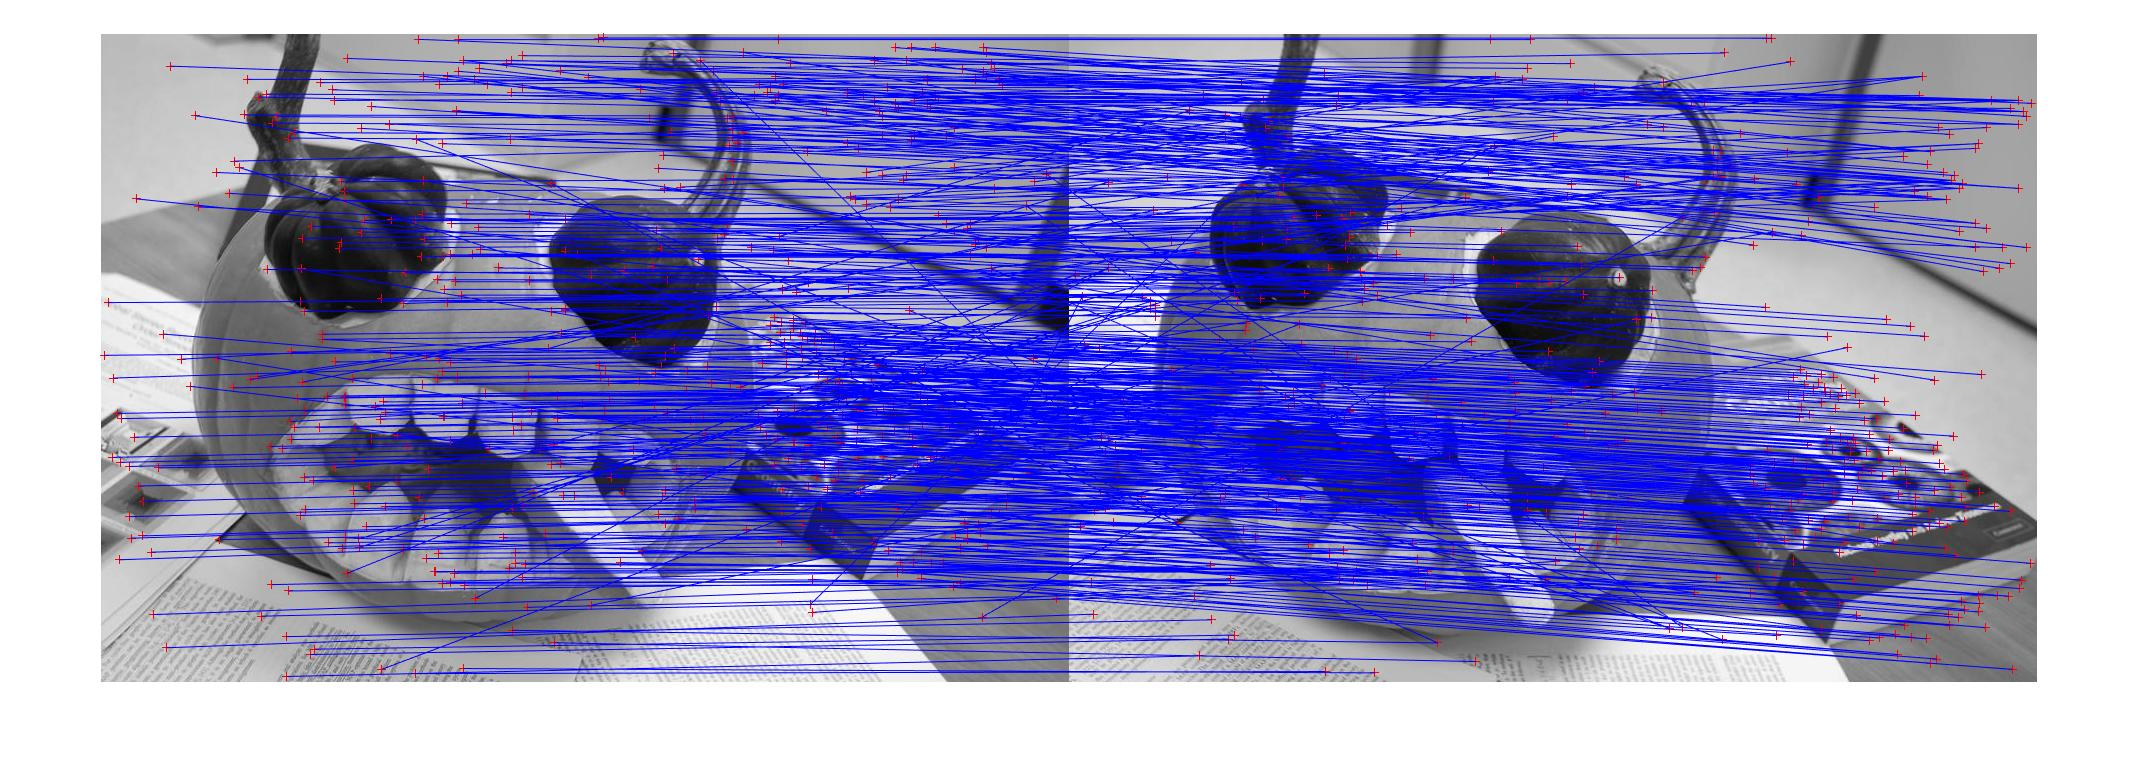
\includegraphics[width=0.8\textwidth]{8r.jpg}
	\caption{point matching before 8 point RANSAC }
	\label{fig1}
\end{figure}
\vspace{5mm}
\newline



\newline
\begin{figure}[ht]
	\centering
	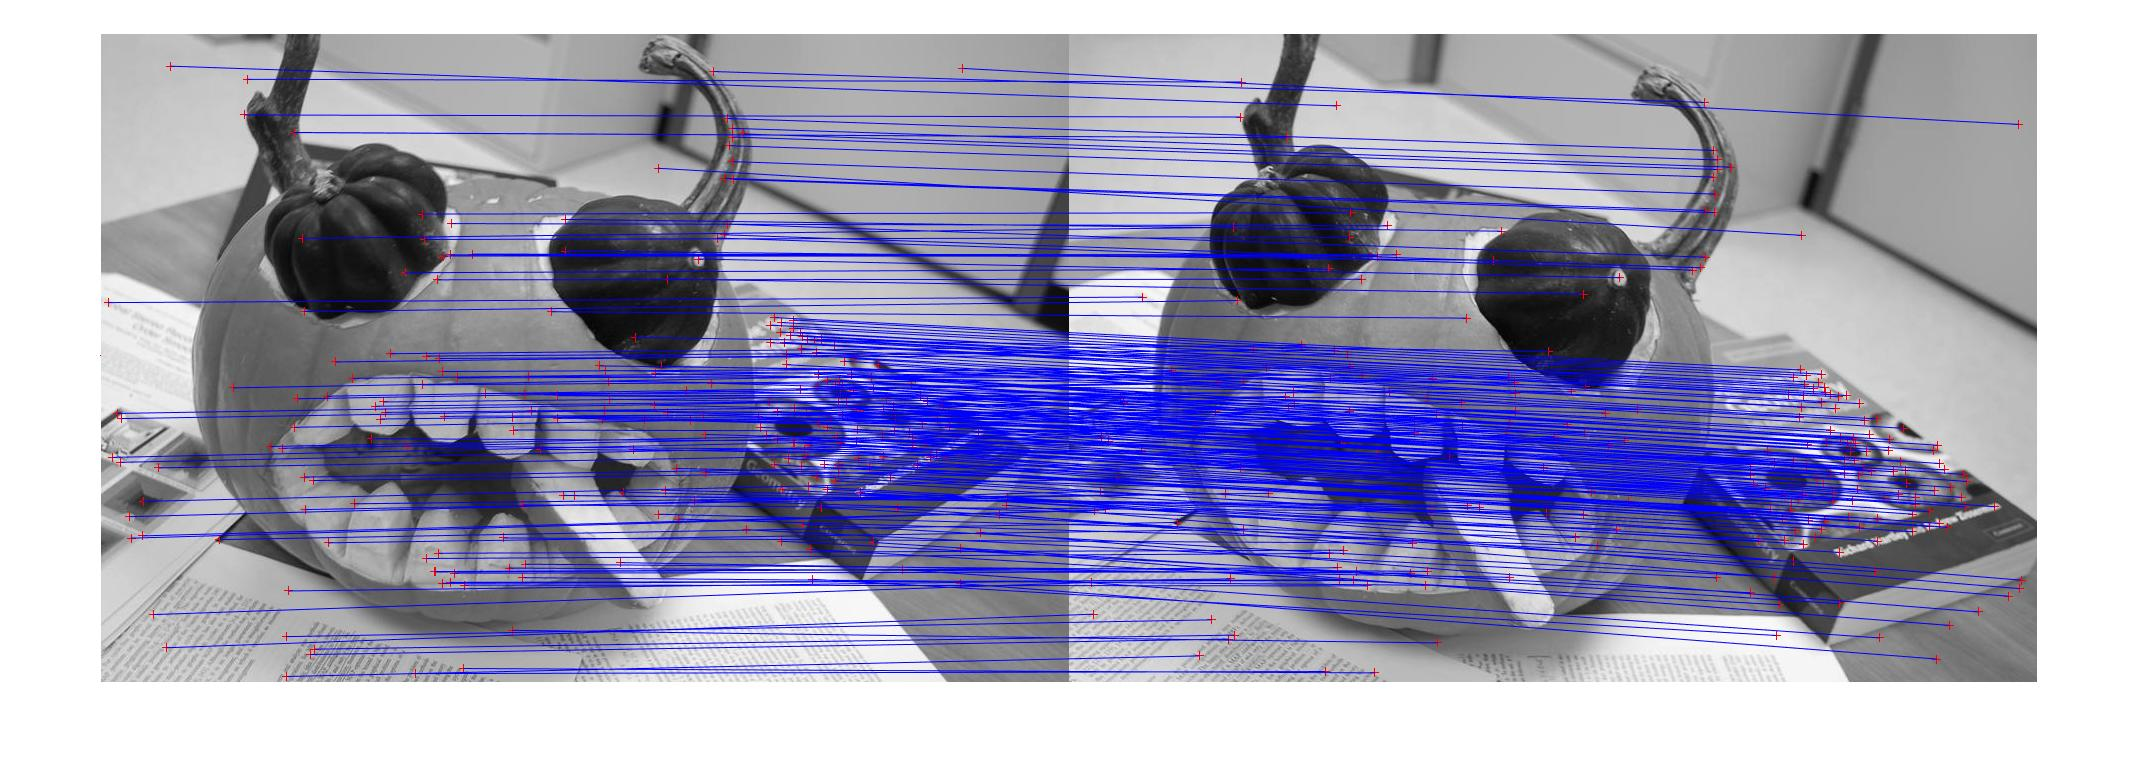
\includegraphics[width=0.8\textwidth]{8r1000_279.jpg}
	\caption{8 point Ransac with M=1000, threshhold =2 and 279 inliers}
	\label{fig1}
\end{figure}
\vspace{5mm}
\newline



\begin{figure}[ht]
	\centering
	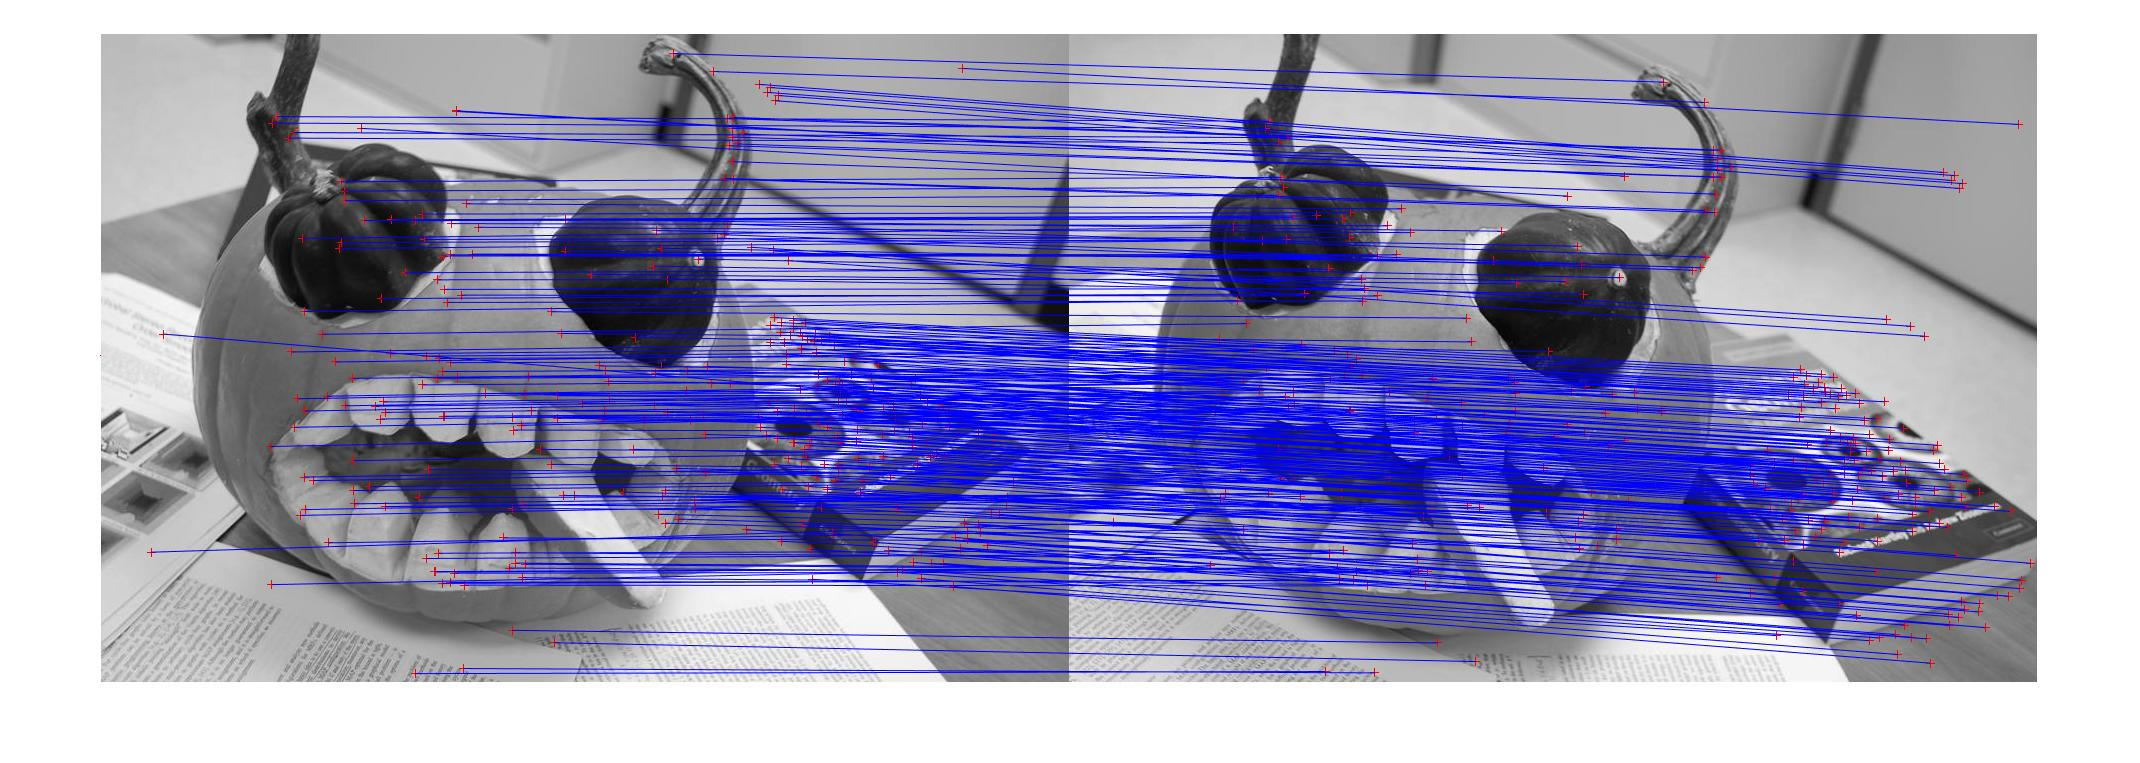
\includegraphics[width=0.8\textwidth]{8r795_344.jpg}
	\caption{8 point Ransac with M=795, threshhold =5 and 344 inliers}
	\label{fig1}
\end{figure}
\vspace{5mm}


\begin{figure}[ht]
	\centering
	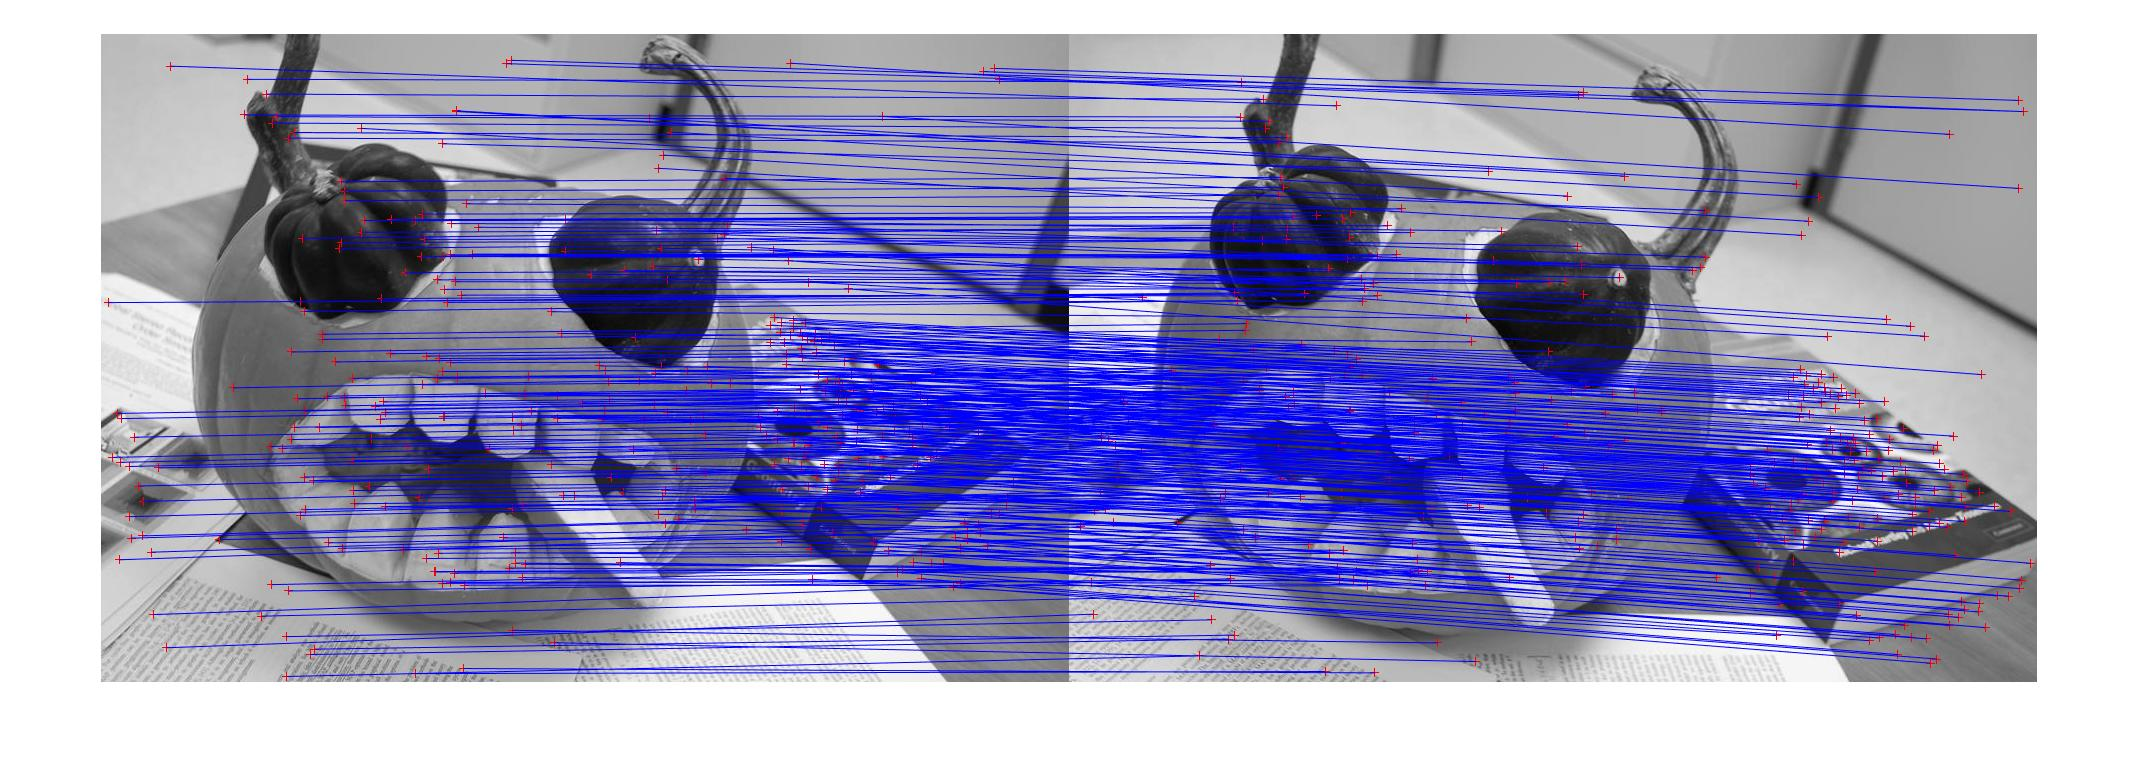
\includegraphics[width=0.8\textwidth]{8r176_399.jpg}
	\caption{8 point Ransac with M=176, threshhold =10 and 399 inliers}
	\label{fig1}
\end{figure}
\vspace{5mm}


\end{document}